% !TEX encoding = UTF-8
% !TEX TS-program = pdflatex
% !TEX root = ../tesi.tex

%**************************************************************
\chapter{Realizzazione}
\label{cap:realizzazione}
%**************************************************************



\section{Studio delle tecnologie}
In questa sezione presento le tecnologie principali utilizzate durante il progetto, cercando di essere quanto più chiaro e sintetico possibile. Questo allo scopo di agevolare la comprensione delle parti finali del capitolo.

\subsection{Realtà aumentata}
La realtà aumentata consiste nel prendere lo spazio tridimensionale reale e trasporlo, tramite tecniche di mappatura, in formato digitale per poi poterci effettuare delle manipolazioni tramite \textit{software}. Ad esempio è possibile, nell'applicazione di Ikea, inquadrare il proprio salotto e posizionarci dei modelli poligonali\footnote{Detti anche \textit{asset} poligonali, prendono questo nome perché nel mondo della modellazione digitale tridimensionale le entità sono composte da triangoli adiacenti tra loro (poligoni appunto) che costruiscono una figura volumetrica. Questo perché il triangolo è la più semplice forma bidimensionale esistente, e quindi la meno esosa da calcolare.} che rappresentano la mobilia venduta dal colosso svedese.\\

\begin{figure}[H]
  \centering
  \includegraphics[width=.3\textwidth]{ikea_ar1}\hspace{20mm}
  \includegraphics[width=.3\textwidth]{ikea_ar2}
  \caption[Ikea realtà aumentata \textit{in-app}]{Tramite l'applicazione di Ikea è possibile posizionare in realtà aumenta sedie o altri mobili.}
\end{figure}


Sebbene sia possibile immaginare lo spazio virtuale come un cubo vuoto all'interno del quale posizionare \textit{asset}, vengono applicate delle semplificazioni logiche per una questione di complessità ed efficienza di calcolo: lo spazio viene processato come una serie di piani bidimensionali sovrapposti a diverse altezze (una sorta di \textit{stack} di battaglie navali) e gli ancoraggi si legano quindi a una coppia di coordinate \textit{(x,y)} relativa al piano più la coordinata \textit{(z)} del piano stesso. I piani vengono divisi in verticali e orizzontali.

\begin{figure}[H]
  \centering
  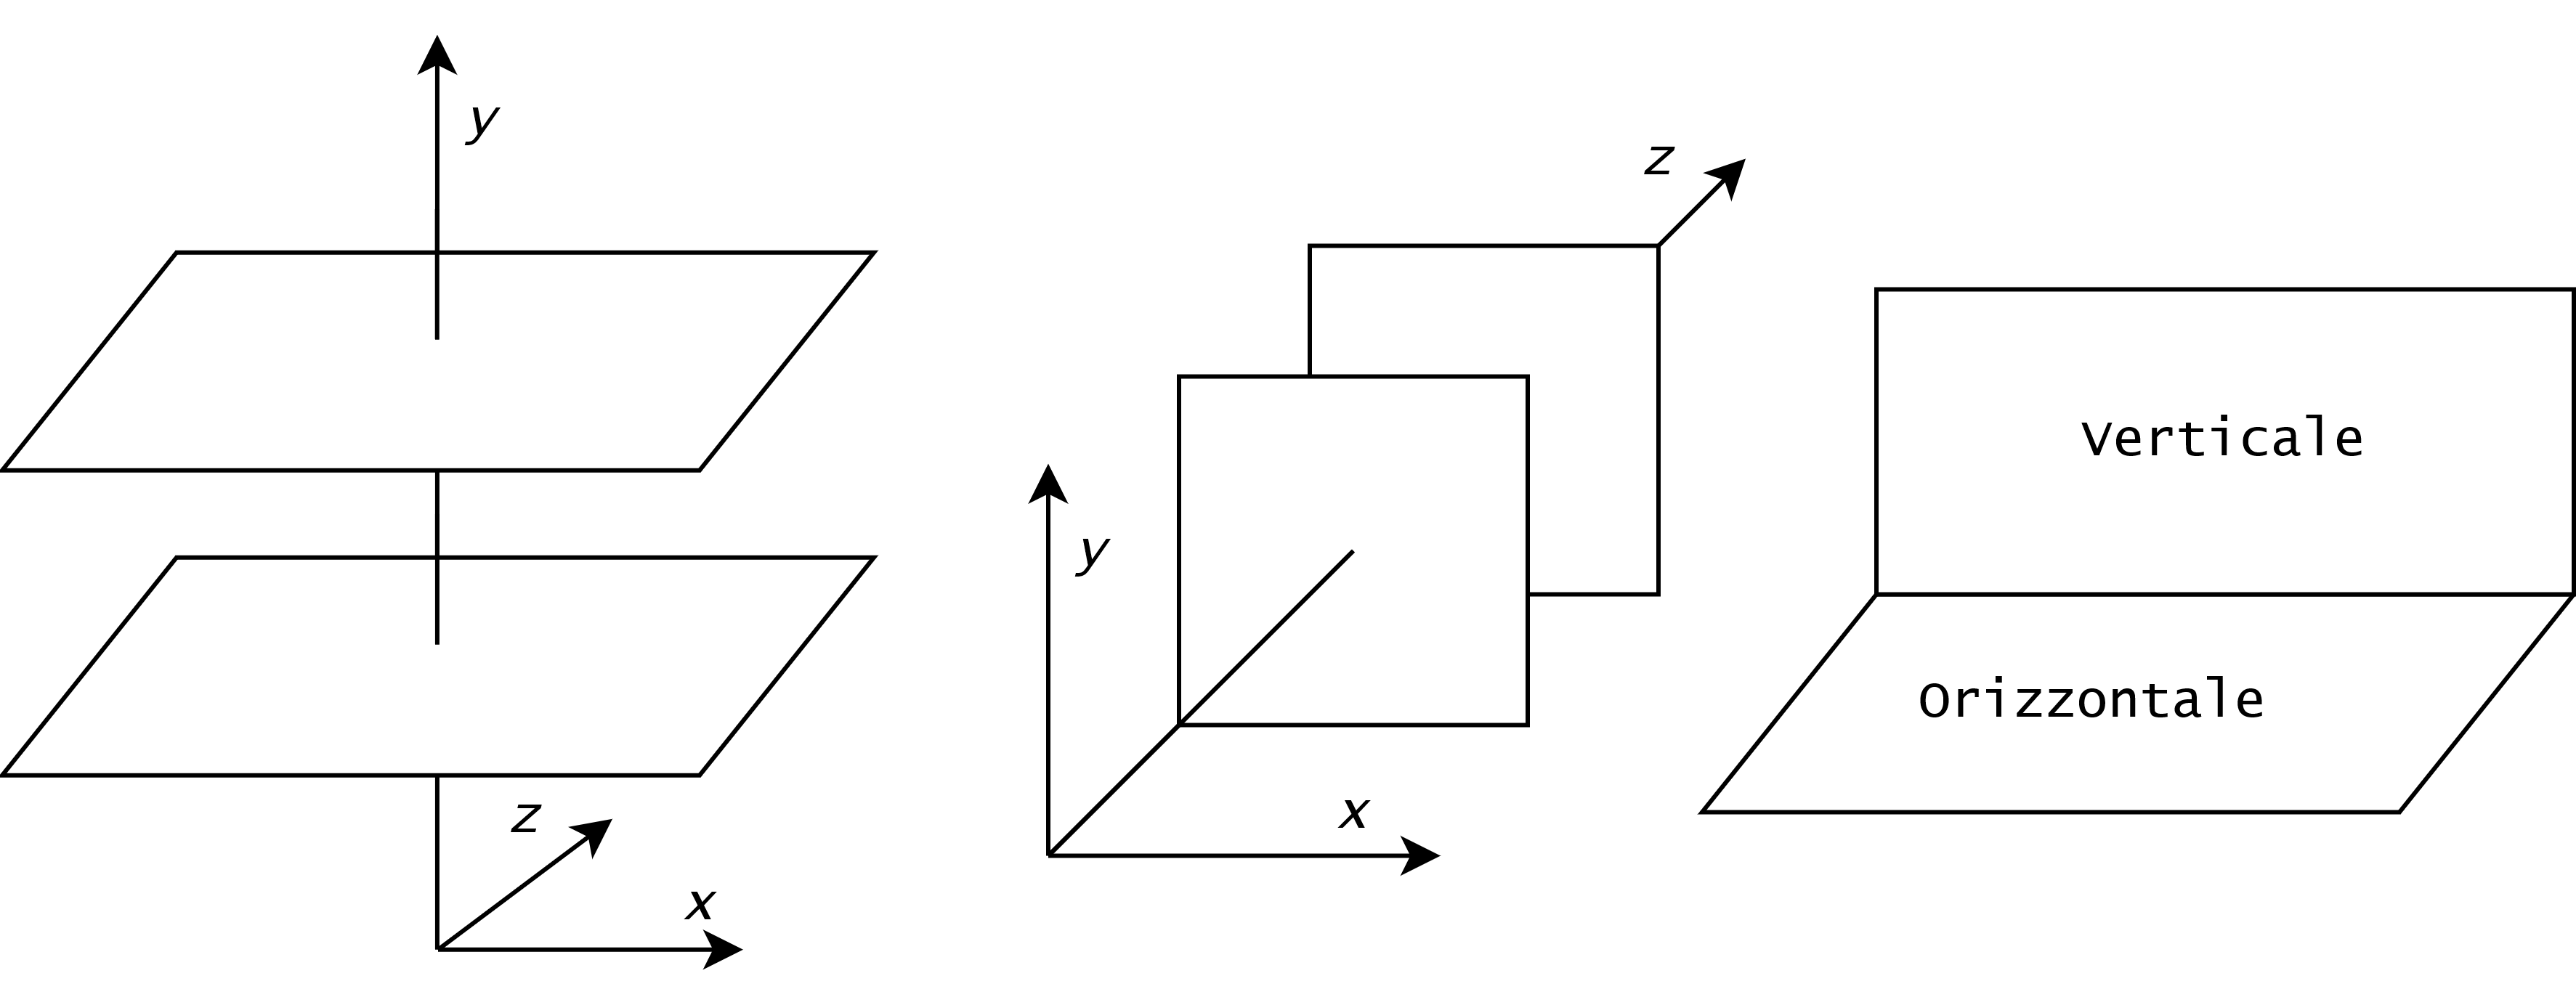
\includegraphics[width=\textwidth]{ar_planes}
  \caption[Piani in realtà aumentata]{In realtà aumentata vengono identificati due tipologie di piano: orizzontale e verticale. Possono essere usati sia singolarmente (prima e seconda figura) che assieme (ultima figura).}
\end{figure}

Nella maggior parte dei casi è bene che oggetti multipli siano legati a un ancoraggio singolo, questo perché la \textit{pose} degli oggetti (ovvero rotazione verticale e orizzontale) è legata a quella della \textit{anchor} associata. Di conseguenza se vogliamo rappresentare in una stanza un insieme realistico di mobili (o meglio, di modelli poligonali e quindi gemelli digitali di mobili), e li leghiamo a un ancoraggio centrale rispetto alla stanza tutti gli elementi avranno sempre una posizione relativa corretta tra loro. Se invece ogni elemento ha la sua \textit{anchor} potremmo vedere rotazioni errate oppure potrebbero spostarsi anche di qualche metro rispetto alla loro posizione originale (entrambi questi scenari vanno intesi in relazione con gli altri ancoraggi e quindi con gli altri oggetti).

\begin{figure}[H]
  \centering
  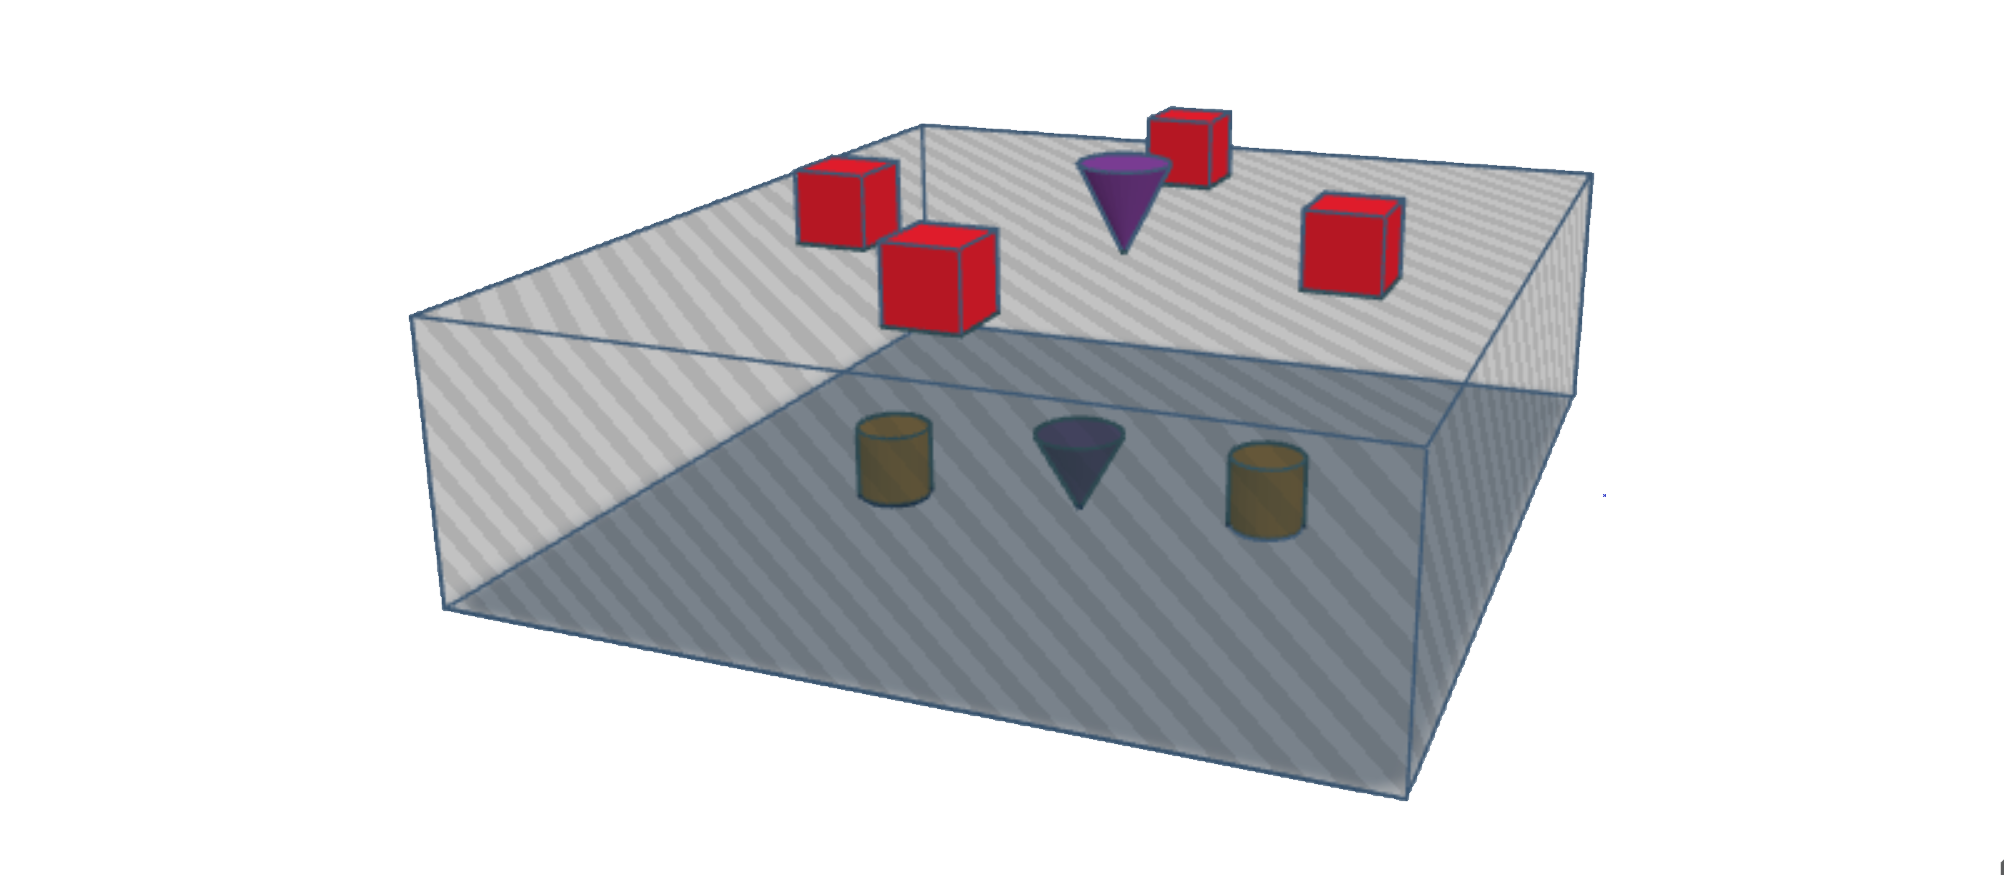
\includegraphics[width=\textwidth]{ancoraggi_multipiano}
  \caption[Ancoraggi singoli per multipli elementi]{A un ancoraggio (in viola) possono essere collegati molteplici elementi (rispettivamente i cubi rossi per l'ancoraggio in alto e i cilindri gialli per quello in basso), e gli ancoraggi possono essere nello stesso spazio ma su due piani diversi.}
\end{figure}

\subsection{Azure ToolKit}
Azure è l'ombrello sotto al quale vivono tutti i servizi \textit{cloud} di Microsoft esterni al pacchetto Office 365, e comprendono \textit{database} relazionali con scalabilità automatica (Azure SQL o Azure Cosmos DB), macchine virtuali remote (Virtual Machines e Azure Virtual Desktop), ma anche funzionalità estremamente avanzate come Azure Kubernetes Service che fornisce un sistema automatizzato per rilasciare, scalare e gestire grandi applicativi \textit{sofware} (ad esempio per i \textit{data center}), oppure Azure Quantum che mette a disposizioni soluzioni per scrivere e provare \textit{software} su \textit{hardware} quantistico.\\
Si nota quindi che la \textit{suite} Azure è indirizzata a utenti altamente specializzati e ancora più spesso a organizzazioni vere e proprie.

\begin{figure}[H]
  \centering
  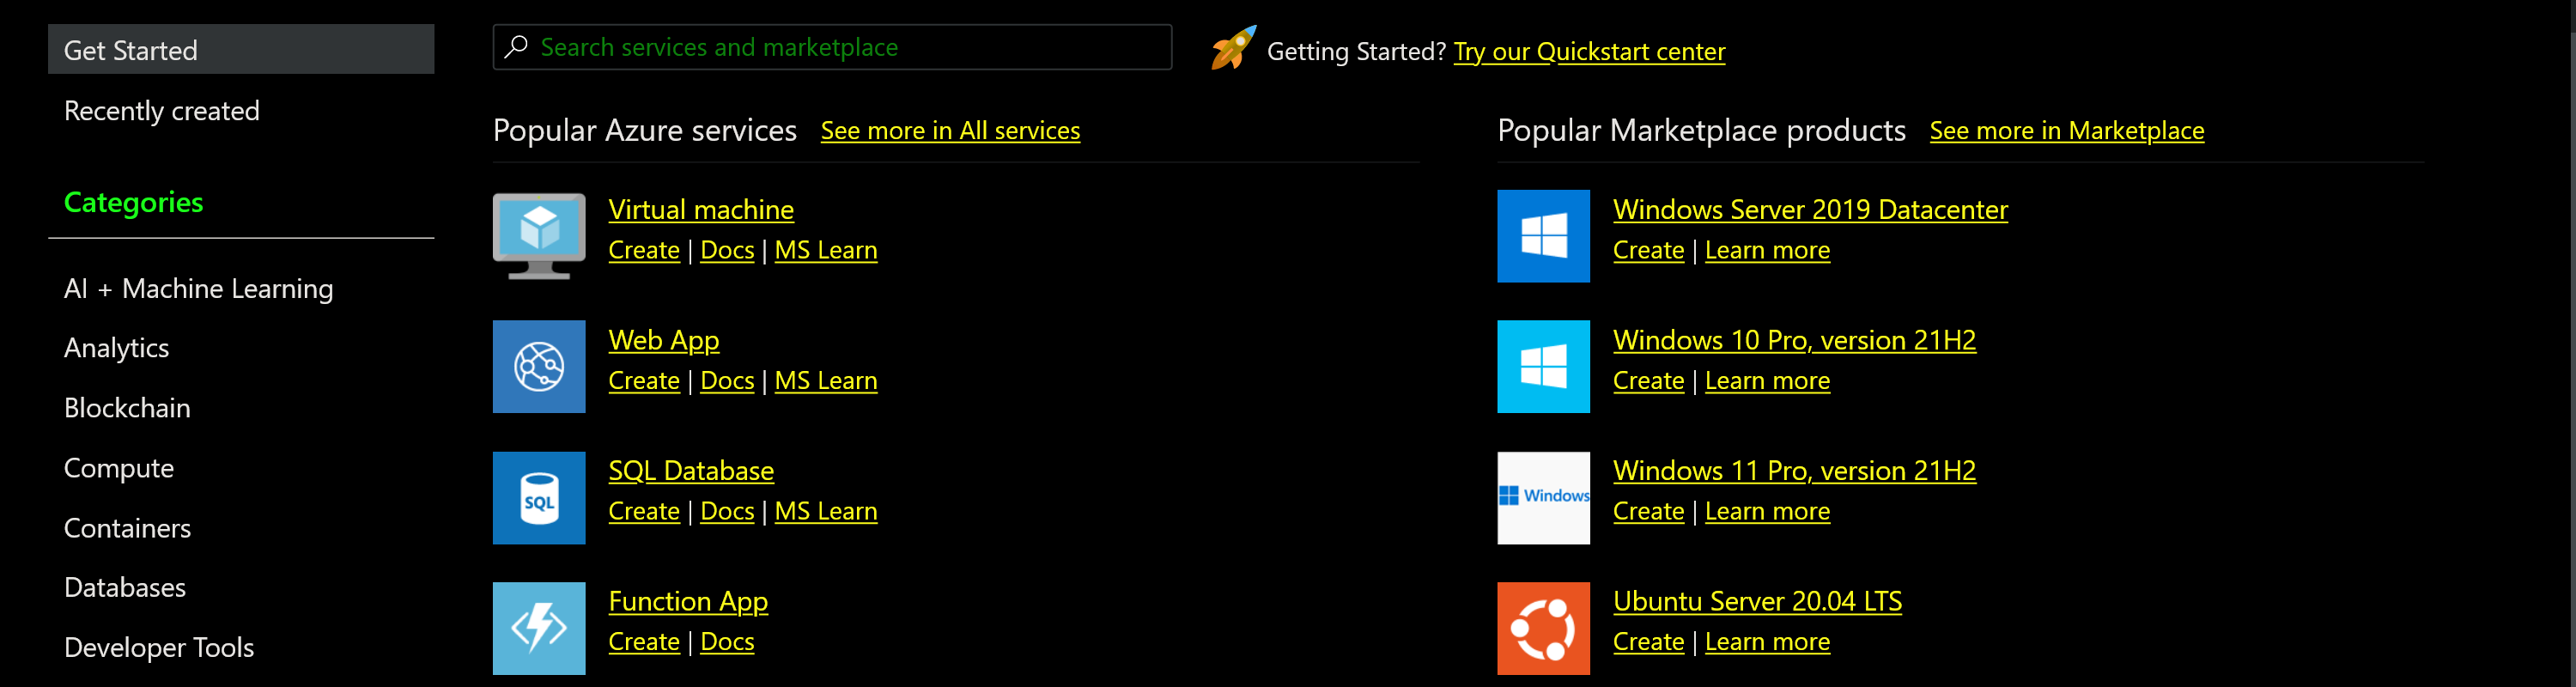
\includegraphics[width=\textwidth]{azure_resources}
  \caption[Azure Portal creazione risorse]{Tramite l'Azure Portal è possibile creare tutte le risorse di Azure, come \textit{server} Ubuntu o macchine virtuali.}
\end{figure}

Per gli scopi di questo progetto ci serviremo di due degli strumenti forniti: l'Azure Portal e le \asa{}.\\
Il primo è semplicemente un portale online che serve a gestire, creare e monitorare tutte le risorse Azure legate a un \textit{account}, mentre le seconde sono il servizio di Microsoft per gestire ancoraggi geospaziali persistenti che possono anche essere utilizzati in un contesto di realtà aumentata.

\begin{figure}[H]
  \centering
  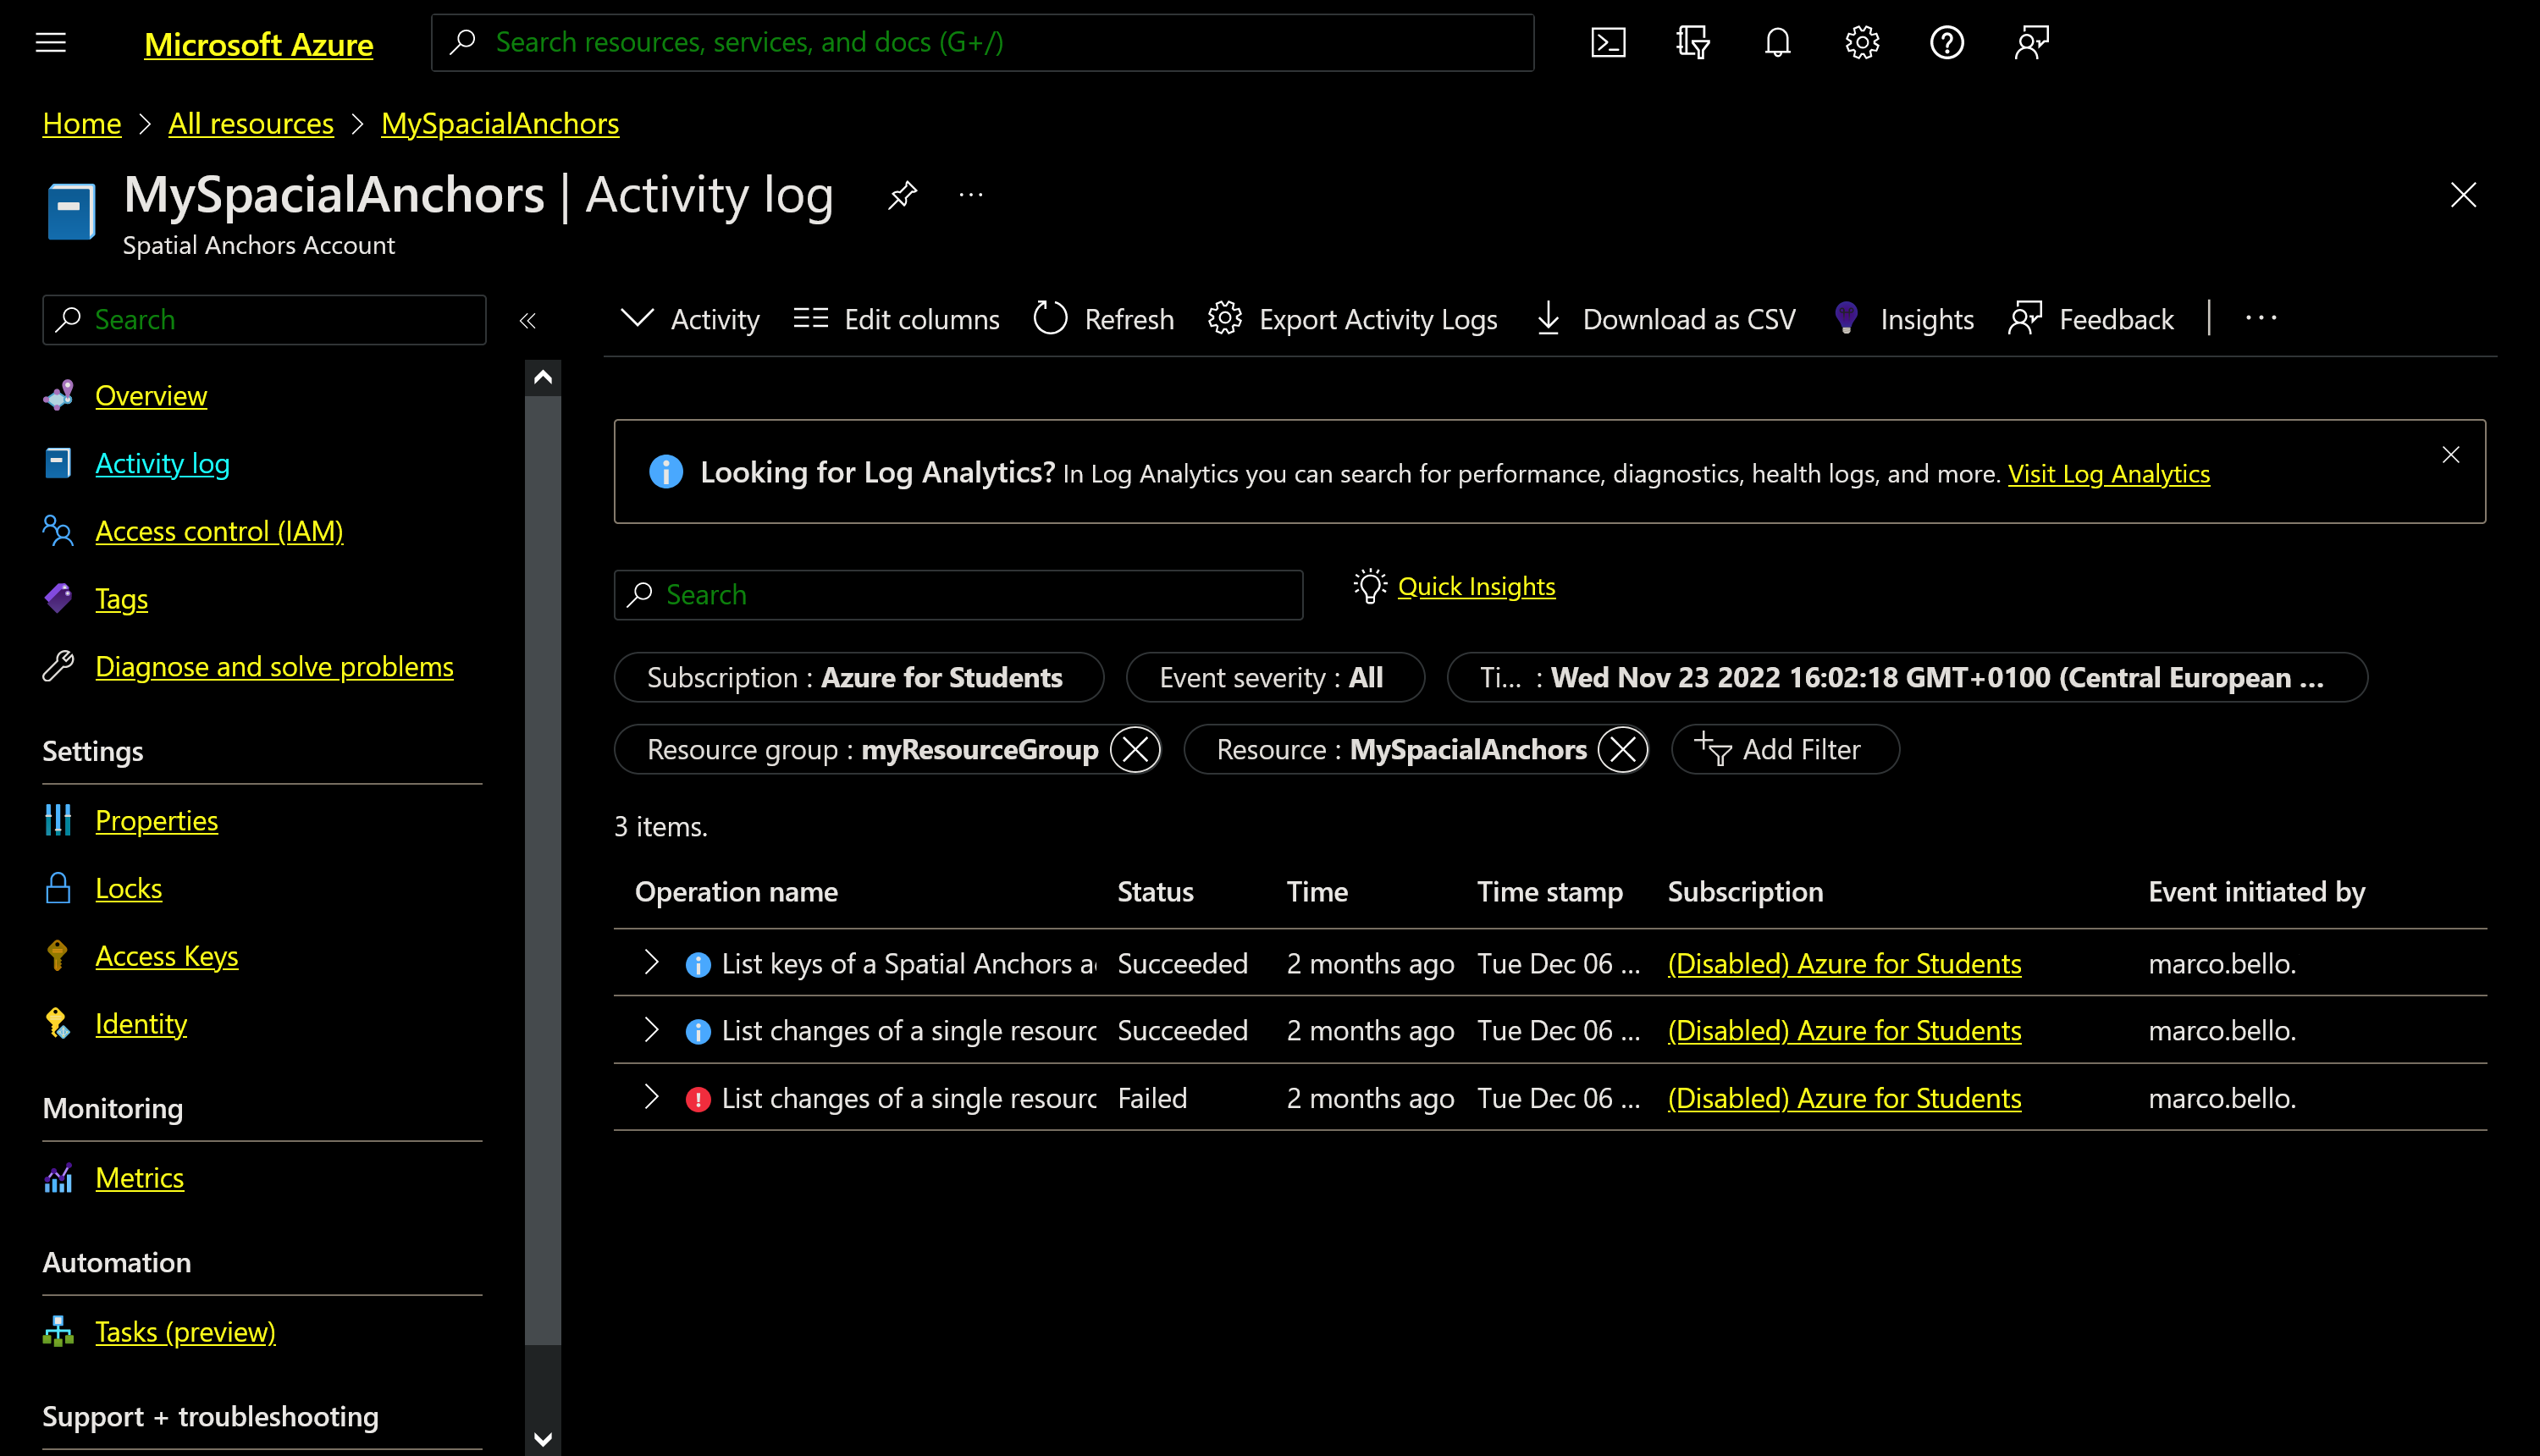
\includegraphics[width=\textwidth]{asa_azure_portal}
  \caption[Azure Portal \asa{}]{Pagina dell'Azure Portal che mostra un dettaglio delle \asa{}, nello specifico il \textit{log} delle attività.}
\end{figure}

Le \asa{} forniscono tre \sdk{}s, uno per Microsoft HoloLens, uno per iOS appoggiandosi su ARKit e uno per Android basato su ARCore, possono collegarsi tra loro creando relazioni che formano dei veri e propri percorsi (funzionalità usata spesso nel contesto degli \textit{asset} aziendali, ad esempio in una stessa linea produttiva) e possono essere contenuti dentro un \textit{resource group} di Azure che funge da contenitore di risorse dentro al quale esse vengono create e gestite.

\subsection{Framework realtà aumentata per Flutter}
Essendo lo scopo di questo stage, e quindi il caso di studio di questa tesi, l'implementazione di una vista in realtà aumentata (nello specifico sfruttando \asa{}) in un'applicazione preesistente sviluppata in Flutter, una grossa parte del lavoro svolto si è incentrato sullo studio dei \textit{framework} e/o \textit{plugin} disponibili.\\
Sfortunatamente, complici la giovinezza di Flutter e la scarsa diffusione di tecnologie per la realtà aumentata, le opzioni sono alquanto ridotte:

\begin{itemize}
    \item \aplug{}: \textit{plugin}\footnote{Fonte: \url{https://pub.dev/packages/ar_flutter_plugin}} che punta a implementare le componenti in realtà aumentata in modalità \textit{cross-platform}, quindi adattandosi autonomamente ad Android e iOS (sfruttando tuttavia le Cloud Anchor di Google). Nasce partendo da due \textit{plugin} più specializzati: 
    \begin{itemize}
        \item arcore\_flutter\_plugin per Android\footnote{Fonte: \url{https://github.com/giandifra/arcore_flutter_plugin}};
        \item arkit\_flutter\_plugin per iOS\footnote{Fonte: \url{https://github.com/olexale/arkit_flutter_plugin}};
    \end{itemize}
    \item ARwayKit: \textit{framework} che mira a fornire un'integrazione semplificata, e in parte già completata, di una componente in realtà aumentata (ottenuta tramite \asa{}) in Flutter tramite vista in Unity.
\end{itemize}

E' necessario notificare che al momento della stesura di questo testo non è più possibile accedere liberamente alla documentazione relativa ad ARwayKit\footnote{Fonte: \url{https://app.gitbook.com/s/-MCtct_TY9f3e8PrcV9T/arwaykit-with-flutter/quickstart-in-flutter}}, tuttavia è ancora reperibile un articolo sul sito Medium che ricalca la guida introduttiva precedentemente fornita dal sito ufficiale dell'azienda\footnote{Fonte: \url{https://medium.com/arway/building-ar-navigation-apps-with-flutter-and-arwaykit-280b69401cd9}}. 
E' anche possibile trovarne una versione nella Wayback Machine\footnote{Fonte: \url{https://web.archive.org/web/20220525060655/https://docs.arway.app/arwaykit-with-flutter/quickstart-in-flutter}}.

\subsubsection{ARWayKit}
ARwayKit è un \textit{framework} formato da un insieme di componenti che si pone l'obiettivo di fornire un'esperienza in realtà aumentata persistente, e lo persegue fornendo un \sdk{} Unity, un'applicazione di mappatura e un insieme di \api{} REST\footnote{Conosciute anche come RESTful API, sono delle \api{} che si conformano allo stile architetturale e alle norme per sistemi distribuiti chiamato \textit{representational state transfer} largamente utilizzato nella comunicazione \textit{web}.}, che implementano le componenti in realtà aumentata in Flutter sfruttando il \textit{plugin} flutter\_unity\_widget\footnote{Fonte: \url{https://pub.dev/packages/flutter_unity_widget}}.\\
E' multipiattaforma, implementa gli ancoraggi tramite \asa{} e funziona in ambienti \textit{"GPS-denied"}, ovvero dove i dati di posizione del \textit{global positioning system}\footnote{Sistema di satelliti in grado di fornire a un ricevitore le sue coordinate geografiche.} non vengono utilizzati per muoversi all'interno dell'ambiente virtuale (oppure ambienti con protocolli di \textit{privacy} elevati). Le caratteristiche appena descritte renderebbero ARwayKit apparentemente perfetto per il caso d'uso specifico di questa tesi. 

\begin{figure}[H]
  \centering
  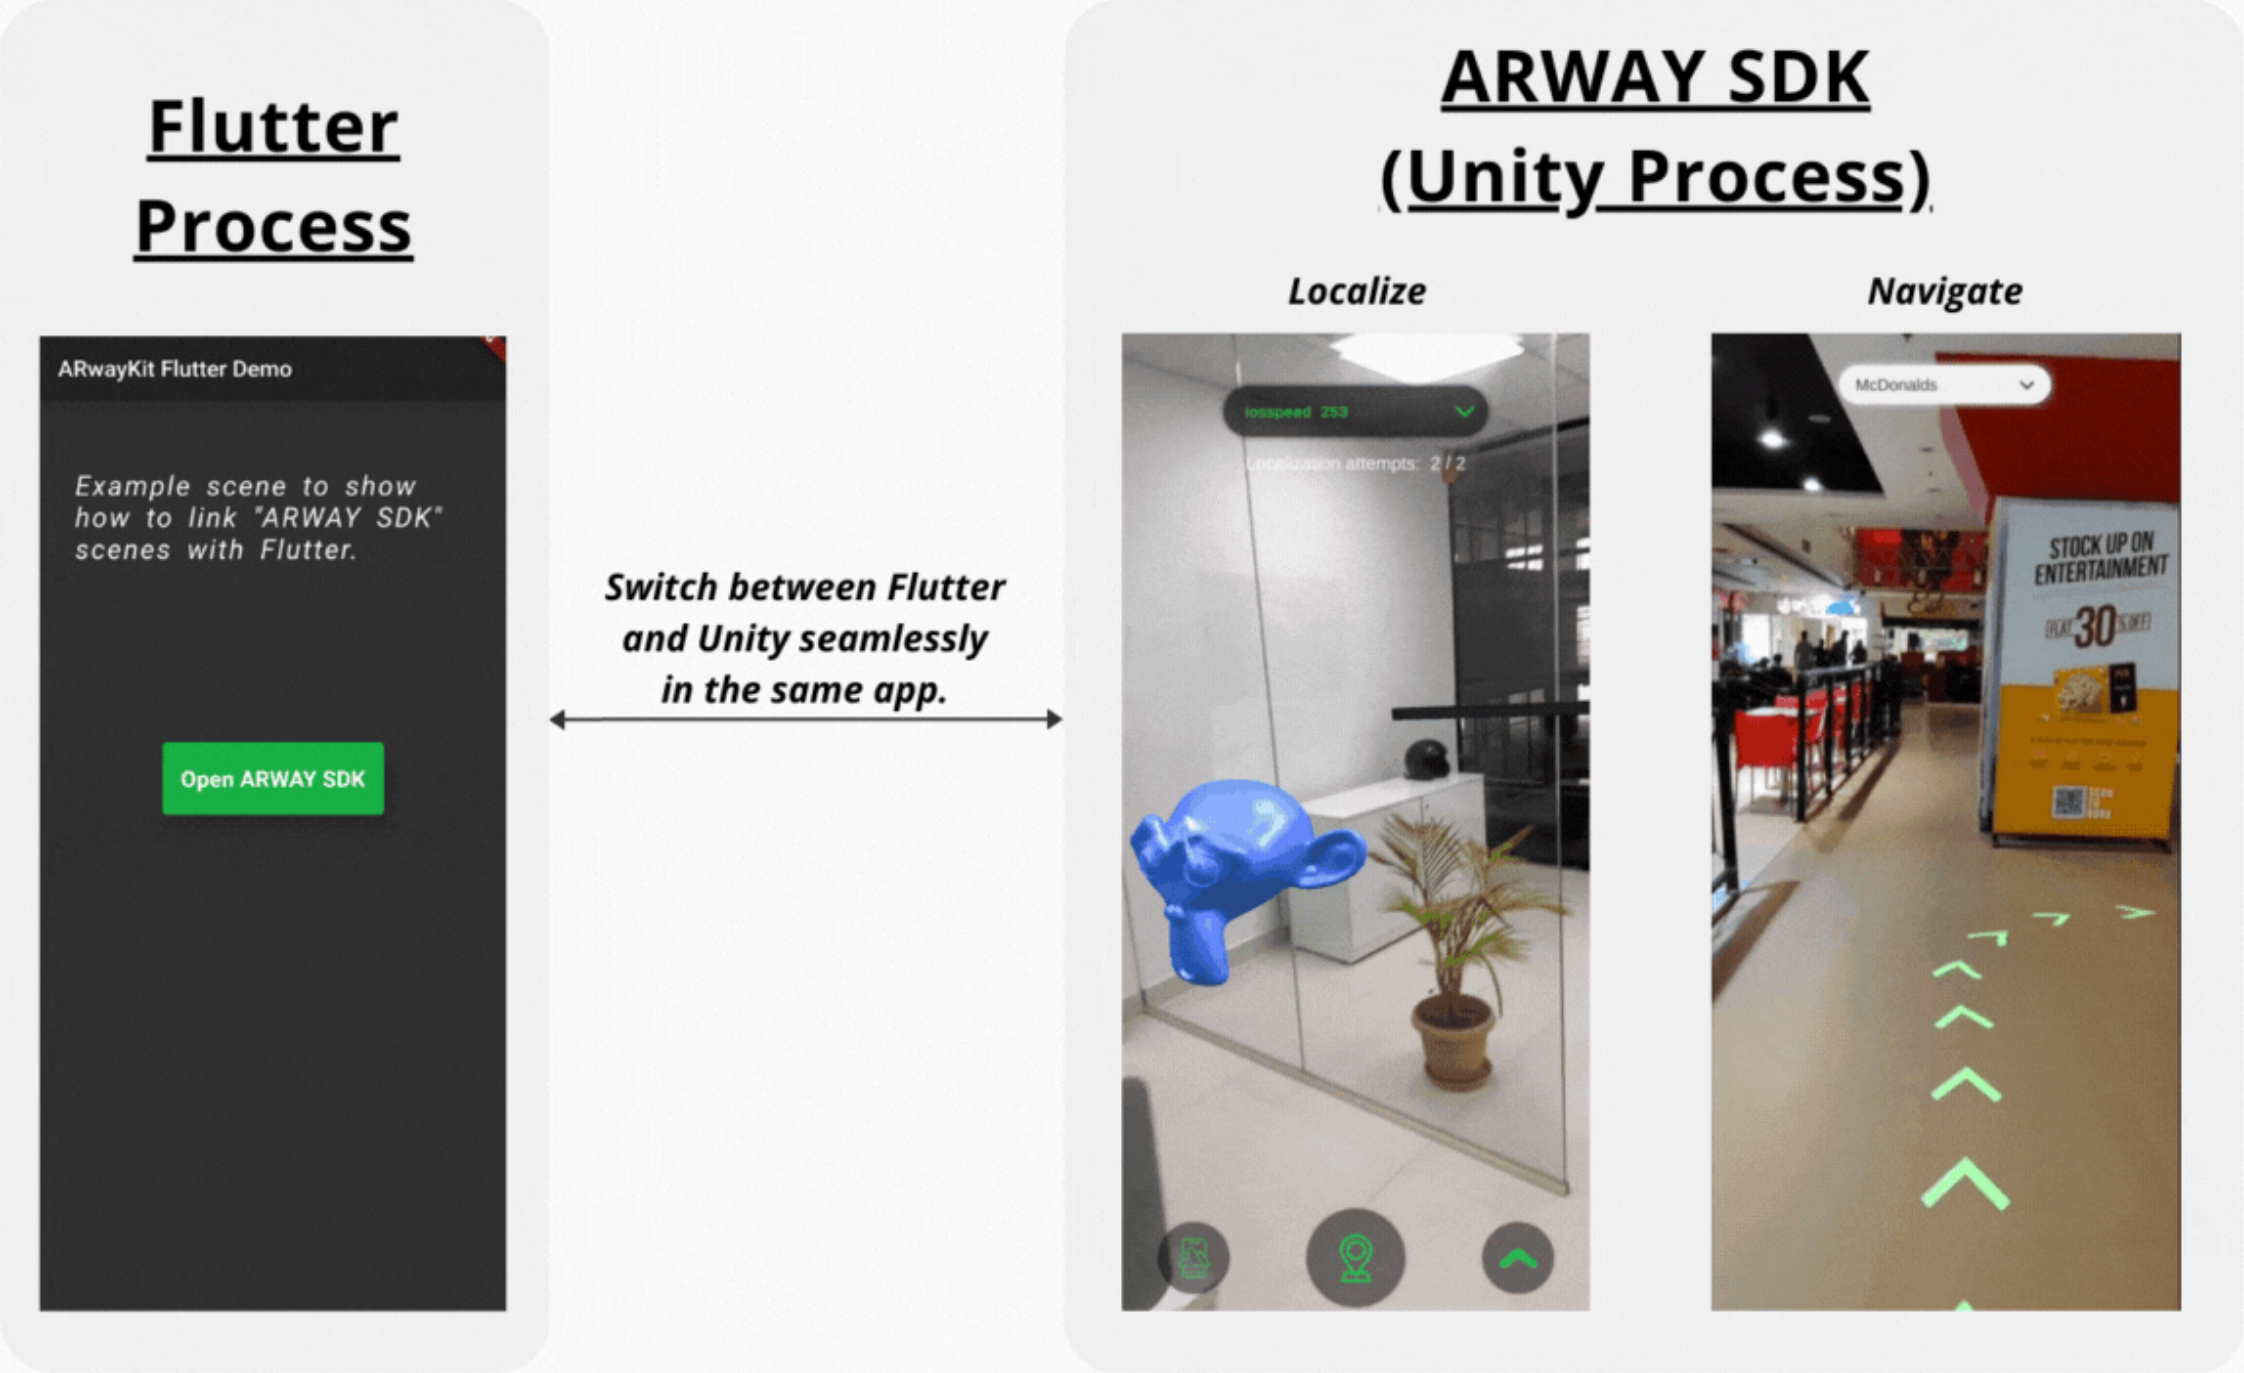
\includegraphics[width=\textwidth]{ARwayKit_samplegif_screenshot}
  \caption[Realtà aumentata con ARwayKit]{Immagine esempio di utilizzo realtà aumentata con ARwayKit\footnotemark}
\end{figure}
\footnotetext{Fonte: \url{https://medium.com/arway/building-ar-navigation-apps-with-flutter-and-arwaykit-280b69401cd9}}

Tuttavia, presenta delle criticità: in primo luogo obbliga l'uso di Unity (sfruttando la sua caratteristica peculiare di poter essere importato come fosse una libreria) per sviluppare la vista in realtà aumentata, il che comporta non solo dover imparare il linguaggio ma dover anche configurare ulteriori componenti (come ad esempio Unity Hub) che poi devono essere adottati assieme a quelli già in uso, appesantendo quindi il processo di codifica.\\
In secondo luogo troviamo invece il problema maggiore: la vista verrebbe realizzata nativamente in Unity, ovvero si tratta di una componente Unity separata rispetto all'applicazione che la lancia.
Questo renderebbe complesso se non impossibile usare dentro essa delle funzionalità Flutter: ad esempio, un bottone a schermo sarebbe un pulsante Unity, non Flutter, obbligando quindi poi a costruire una mappatura tra i due linguaggi per ogni funzionalità visualizzata.\\ 
Una vista così costruita non solo è scomoda da programmare, ma anche difficile da manutenere.

\subsubsection{ar\_flutter\_plugin}
\aplug{} è un \textit{plugin open-source} collaborativo estremamente giovane (il primo \textit{commit} sulla \textit{repository} pubblica risale al 6 febbraio 2021\footnote{Fonte: \url{https://github.com/CariusLars/ar_flutter_plugin/commit/da9ab148219d833755ef7a9b1e3536a3cae865d1}}) che si pone l'obiettivo di implementare componenti in realtà aumentata in Flutter.\\
Per raggiungere lo scopo si serve della libreria archiviata Sceneform\footnote{Fonte: \url{https://developers.google.com/sceneform/develop}}, che si occupa di "renderizzare scene tridimensionali realistiche in applicazioni in realtà aumentata o meno, senza dover imparare OpenGL".\\

\begin{figure}[H]
  \centering
  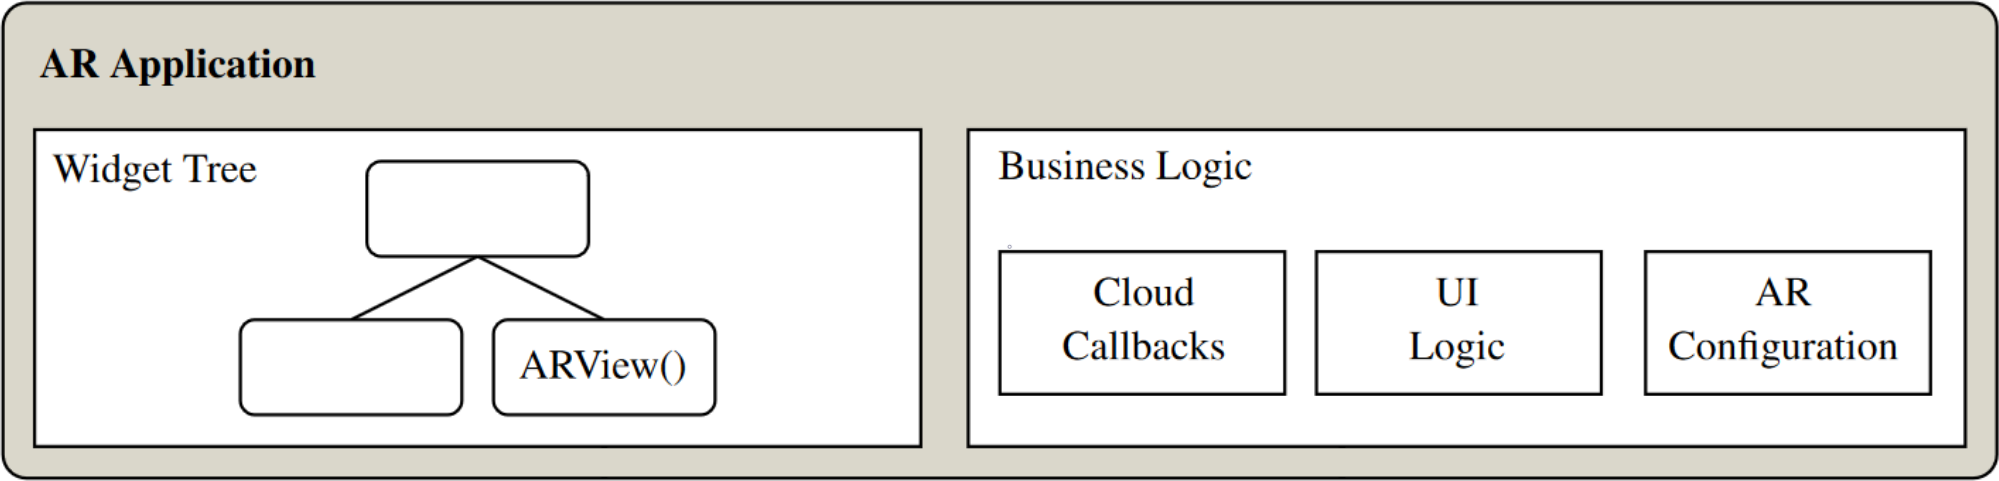
\includegraphics[width=\textwidth]{carsius1}
  \caption[Applicazione realtà aumentata \aplug{}]{Schematizzazione applicazione cliente per \aplug{}.\footnotemark}
\end{figure}
\footnotetext{Fonte: \url{https://lars.carius.io/blog/ar_flutter_plugin.html}}

L'architettura di \aplug{} è composta da due componenti: delle \api{} multipiattaforma unificate che forniscono un'interfaccia alle applicazioni tramite il \textit{plugin} e le implementazioni specifiche per le piattaforme Android (in Kotlin) e iOS (in Swift) costruite su ARCore e ARKit rispettivamente, così da garantire accesso continuativo nel tempo a funzionalità aggiornate.\\
\aplug{} espone dei \textit{widget} che possono essere inclusi nel \textit{widget tree} dell'applicazione cliente e delle classi \textit{manager} per gestire funzionalità e logiche di controllo del \textit{plugin} e delle componenti in realtà aumentata: \textit{session manager}, \textit{object manager}, \textit{anchor manager} e \textit{location manager}.\\ 
Il \textit{session manager} gestisce le configurazioni di tracciamento (ad esempio se usare piani orizzontali, verticali o entrambi), opzioni di \textit{debugging} (come la visualizzazione dei piani) e le \textit{callbacks} per gli \textit{hit-test}\footnote{Immaginando un vettore che parte dall'ottica del dispositivo e tocca una superficie, possiamo considerare quel contatto un \textit{"hit"}. Con \textit{hit-testing} si intende valutare la capacità di tracciare correttamente lo spazio inteso come distanza tra i punti dello stesso e il dispositivo.} e i \textit{gesture events}\footnote{Azioni che il sistema deve fare quando vengono effettuati degli \textit{input} tramite \textit{touch screen} del dispositivo}.\\

\begin{figure}[H]
  \centering
  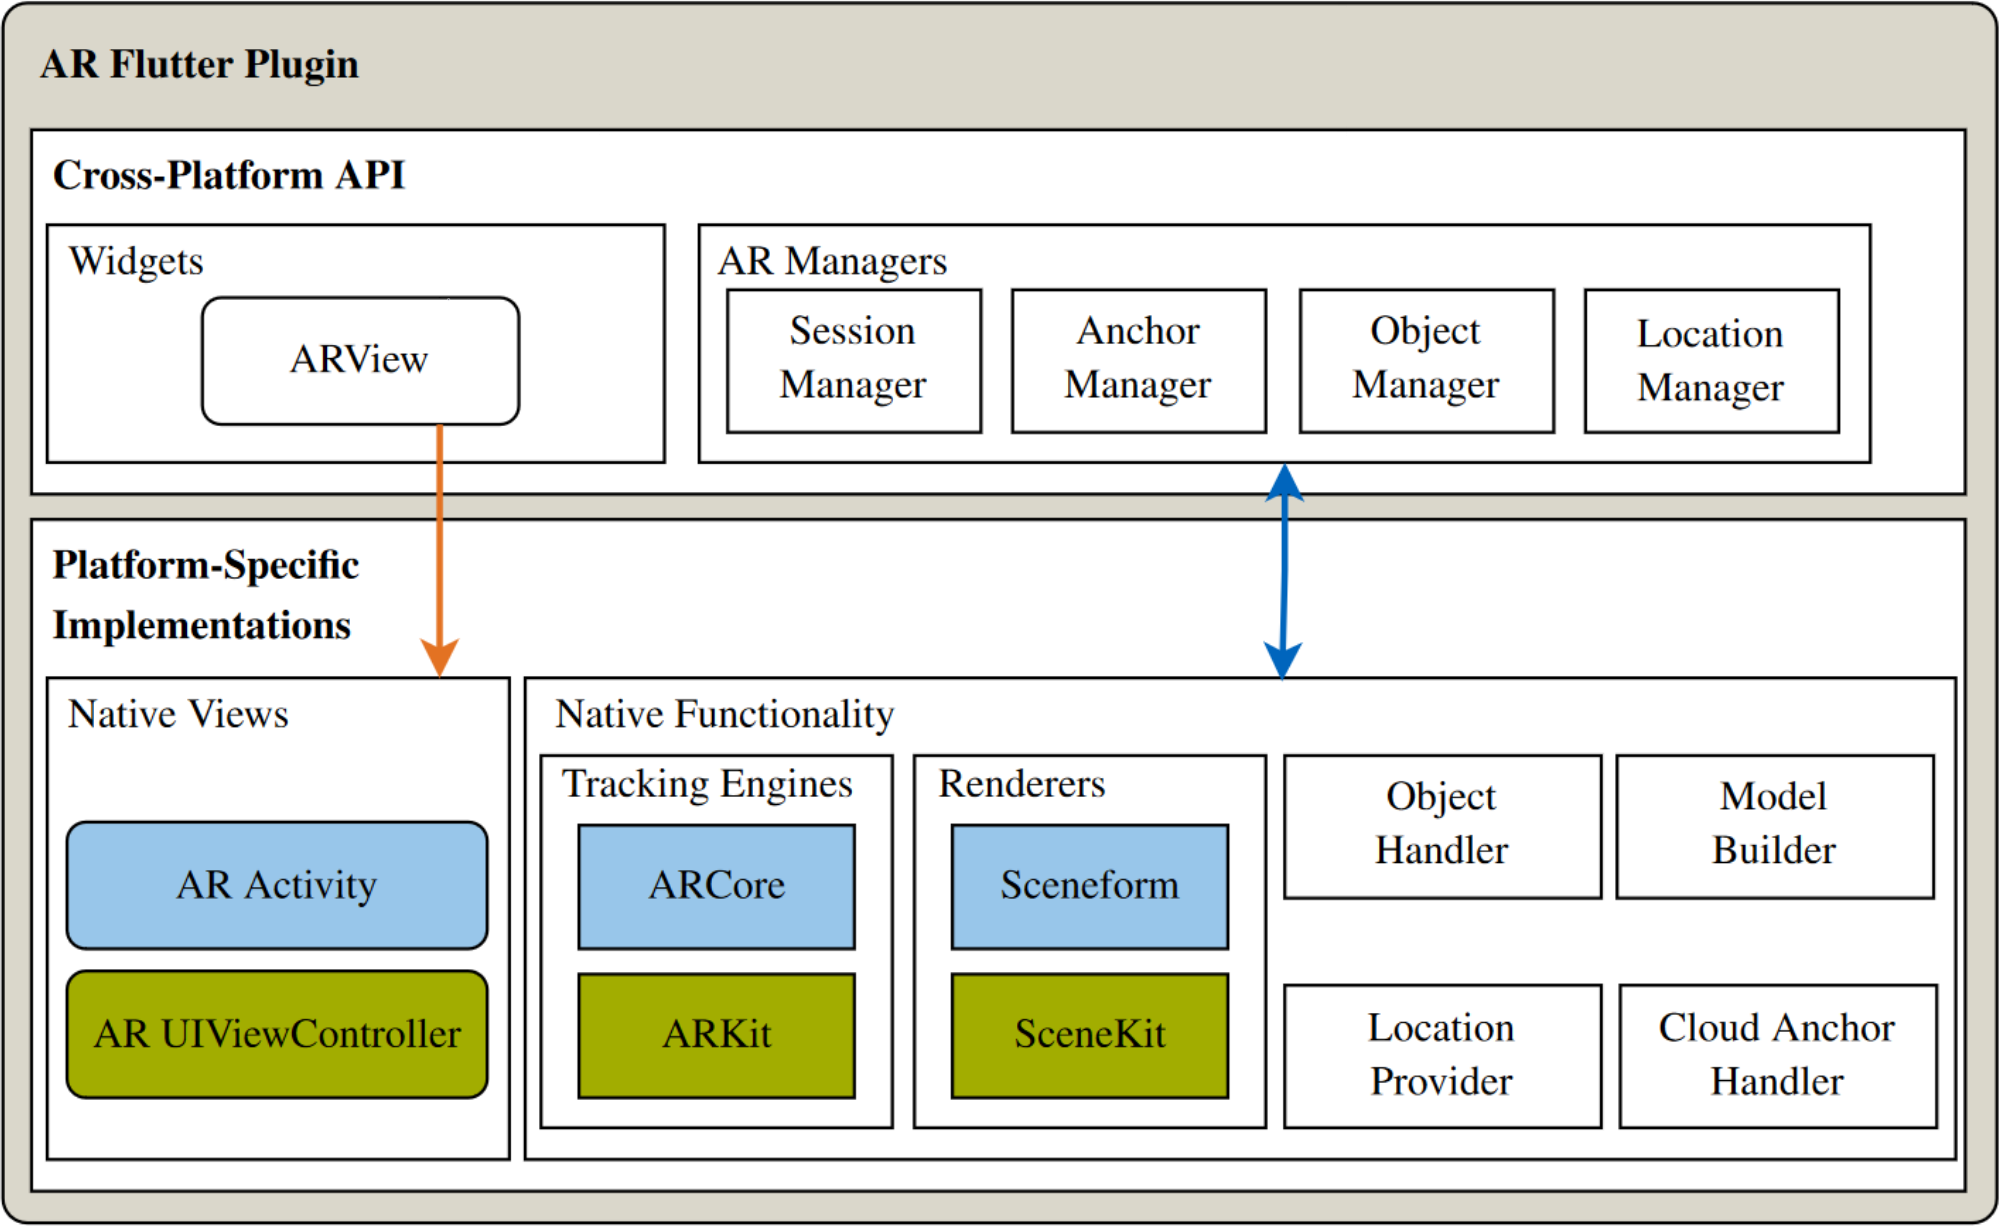
\includegraphics[width=\textwidth]{carsius2}
  \caption[Schema \aplug{}]{Schematizzazione logica interna di \aplug{}.\footnotemark}
\end{figure}
\footnotetext{Fonte: \url{https://lars.carius.io/blog/ar_flutter_plugin.html}}

L'\textit{object manager} gestisce i nodi (le entità) in realtà aumentata del \textit{plugin} che servono ad astrarre rispetto alle funzionalità native delle varie piattaforme (ARCore e ARKit ad esempio) e permettono di aggiungere, modificare o rimuovere nodi basandosi su formati GLTF2 o GLB che possono essere caricati a \textit{runtime} da un \textit{file system} o dalla rete.\\
L'\textit{anchor manager} contiene funzioni per caricare e ottenere ancoraggi da servizi \textit{cloud} servendosi delle \api{} fornite da Google Coud Anchor. Gli ambienti virtuali registrati localmente possono essere salvati in rete e comparati con quelli già in \textit{storage} persistente per scaricare ancoraggi e oggetti precedentemente posizionati nella scena.\\
Infine il \textit{location manager} si occupa di fornire le coordinate del \textit{global positioning system}  per permettere un'interrogazione efficiente degli ancoraggi basati su posizione geografica.\\
Il \textit{plugin} ha un'architettura largamente \textit{clout-agnostic}, cioè non si interessa dell'implementazione specifica per i servizi di salvataggio persistente, il che gli permette di usare facilmente gestori di contenuti esterni.

\subsubsection{Confronto}
Vediamo quindi di schematizzare e mettere a confronto pregi e difetti delle due soluzioni trovate.\aCapo{}

\textbf{Pregi ARwayKit:}
\begin{itemize}
  \item Implementa nativamente le \asa{};
  \item Funziona in ambienti \textit{GPS-denied};
  \item E' pensato per uso aziendale.
\end{itemize}

\textbf{Difetti ARwayKit:}
\begin{itemize}
  \item La vista e le componenti in realtà aumentata non sono implementate in Flutter;
  \item Richiede l'uso di Unity che, essendo un motore per videogiochi, ha funzionalità in più (e in meno) non necessarie (e necessarie) rispetto a un uso aziendale;
  \item Ha una documentazione difficile da reperire e di dubbia completezza;
  \item E' codice propietario, quindi non c'è modo di visionare il sorgente.
\end{itemize}

\textbf{Pregi \aplug{}:}
\begin{itemize}
  \item La vista e le componenti in realtà aumentata sono implementate in Flutter;
  \item Ha un documentazione discreta;
  \item E' \textit{open-source}, quindi al bisogno è possibile visionare il codice sorgente;
  \item E' pensato per uso aziendale;
  \item La struttura logica, divisa nei vari \textit{manager}, è modulare e chiara da comprendere, il che dovrebbe facilitarne modifica ed estensione;
  \item Promette di essere \textit{cloud-agnostic}, quindi favorisce l'uso di gestorie sterni come ad esempio \asa{} 
\end{itemize}

\textbf{Difetti \aplug{}:}
\begin{itemize}
  \item Non implementa nativamente le \asa{}, usando invece le Google Cloud Anchors;
  \item Non è chiaro se funzioni nativamente in ambienti \textit{GPS-denied};
\end{itemize}

\textbf{Confronto schematico:}

{
  \setlength{\freewidth}{\dimexpr\textwidth-10\tabcolsep}
  \renewcommand{\arraystretch}{1.5}
  \centering
  \setlength{\aboverulesep}{0pt}
  \setlength{\belowrulesep}{0pt}
  \begin{longtable}{C{.6\freewidth} C{.2\freewidth} C{.2\freewidth}} 
     \toprule 
  \cellcolor{red}\textcolor{white}{\textbf{Caratteristica}} &
  \cellcolor{red}\textcolor{white}{\textbf{ARwayKit}} &
  \cellcolor{red}\textcolor{white}{\textbf{Plugin}}\\
  \midrule
  \endhead
  
  \cellcolor{black!20}\asa{} native & \cellcolor{green!20}SI & \cellcolor{red!20}NO\\
  \cellcolor{black!20}Ambienti \textit{GPS-denied} & \cellcolor{green!20}SI & \cellcolor{orange!20}NON CHIARO\\
  \cellcolor{black!20}Vista realtà aumentata implementata in Flutter & \cellcolor{red!20}NO & \cellcolor{green!20}SI\\
  \cellcolor{black!20}Codice sorgente visibile & \cellcolor{red!20}NO & \cellcolor{green!20}SI\\
  \cellcolor{black!20}Pensato per uso aziendale & \cellcolor{green!20}SI & \cellcolor{green!20}SI\\

  \bottomrule
  \rowcolor{white} 
  \caption{Confronto \textit{framework} per realtà aumentata}
  \end{longtable}
}

E' stato infine scelto \aplug{} rispetto ad ARwayKit per evitare di interfacciarsi con Unity, per la necessità di avere la vista in realtà aumentata implementata direttamente in Flutter e per il grande vantaggio che comporta il suo essere \textit{open-source}.

\section{Difficoltà incontrate}
\label{sec:difficolta_incontrate}
Le prime difficoltà incontrate a livello personale sono state di tipo tecnologico: non mi ero mai trovato a programmare con linguaggi orientati al \textit{frontend}, e ho dovuto quindi cambiare almeno in parte il mio \textit{modus operandi} nella progettazione e scrittura di codice. A questo si è aggiunta la necessità di gestire altri tre linguaggi per le implementazioni native, ovvero Java e Kotlin per il lato Android e Swift per la parte iOS e, a complicare le cose, tutti questi linguaggi dovevano essere messi in comunicazione diretta con Flutter (e nel caso di Java e Kotlin anche tra di loro).\\ 
Una buona parte dello \textit{stage} è quindi stata investita nel comprendere e nel gestire la grande diversità di linguaggi diversi.

\begin{figure}[H]
  \centering
  %\includegraphics[height=5cm]{screen_mobilesyn}
  
\includegraphics[width=.5\textwidth]{asa_google_search}\hfill
  
\includegraphics[width=.5\textwidth]{flutter_google_search}\\
  
\includegraphics[width=1\textwidth]{asa_flutter_google_search}
  \caption[Ricerca esatta Flutter e ASA 23 novembre]{Al 23 novembre 2022, una ricerca esatta di "flutter" mostra 87.5 milioni di risultati rilevanti, di "azure spatial anchors" 41 milioni mentre la combinazione delle due, solo 17}
\label{fig:search1}
\end{figure}

In linea più generale invece le due problematiche che hanno più di tutte complicato i lavori (sia per me che per Datasoil stessa) sono stati la mancanza di documentazione adeguata e la mancanza di supporto da parte della comunità degli sviluppatori.\\
Microsoft non fornisce un \textit{set} documentale adeguato per quanto riguarda \asa{}, mostrando il meno possibile della struttura interna (ad esempio come viene rappresentato un ancoraggio) e fornendo solo \api{} per effettuare operazioni ad alto livello (come il salvataggio in \textit{cloud} di un'\textit{anchor}), inoltre la ricerca della documentazione è macchinosa.\\
L'altro problema risiede nella difficoltà estrema di trovare supporto di terze parti (ad esempio in siti come \url{https://stackoverflow.com}), come viene mostrato nelle figure \ref{fig:search1} e \ref{fig:search2}.

\begin{figure}[H]
  \centering
  %\includegraphics[height=5cm]{screen_mobilesyn}
  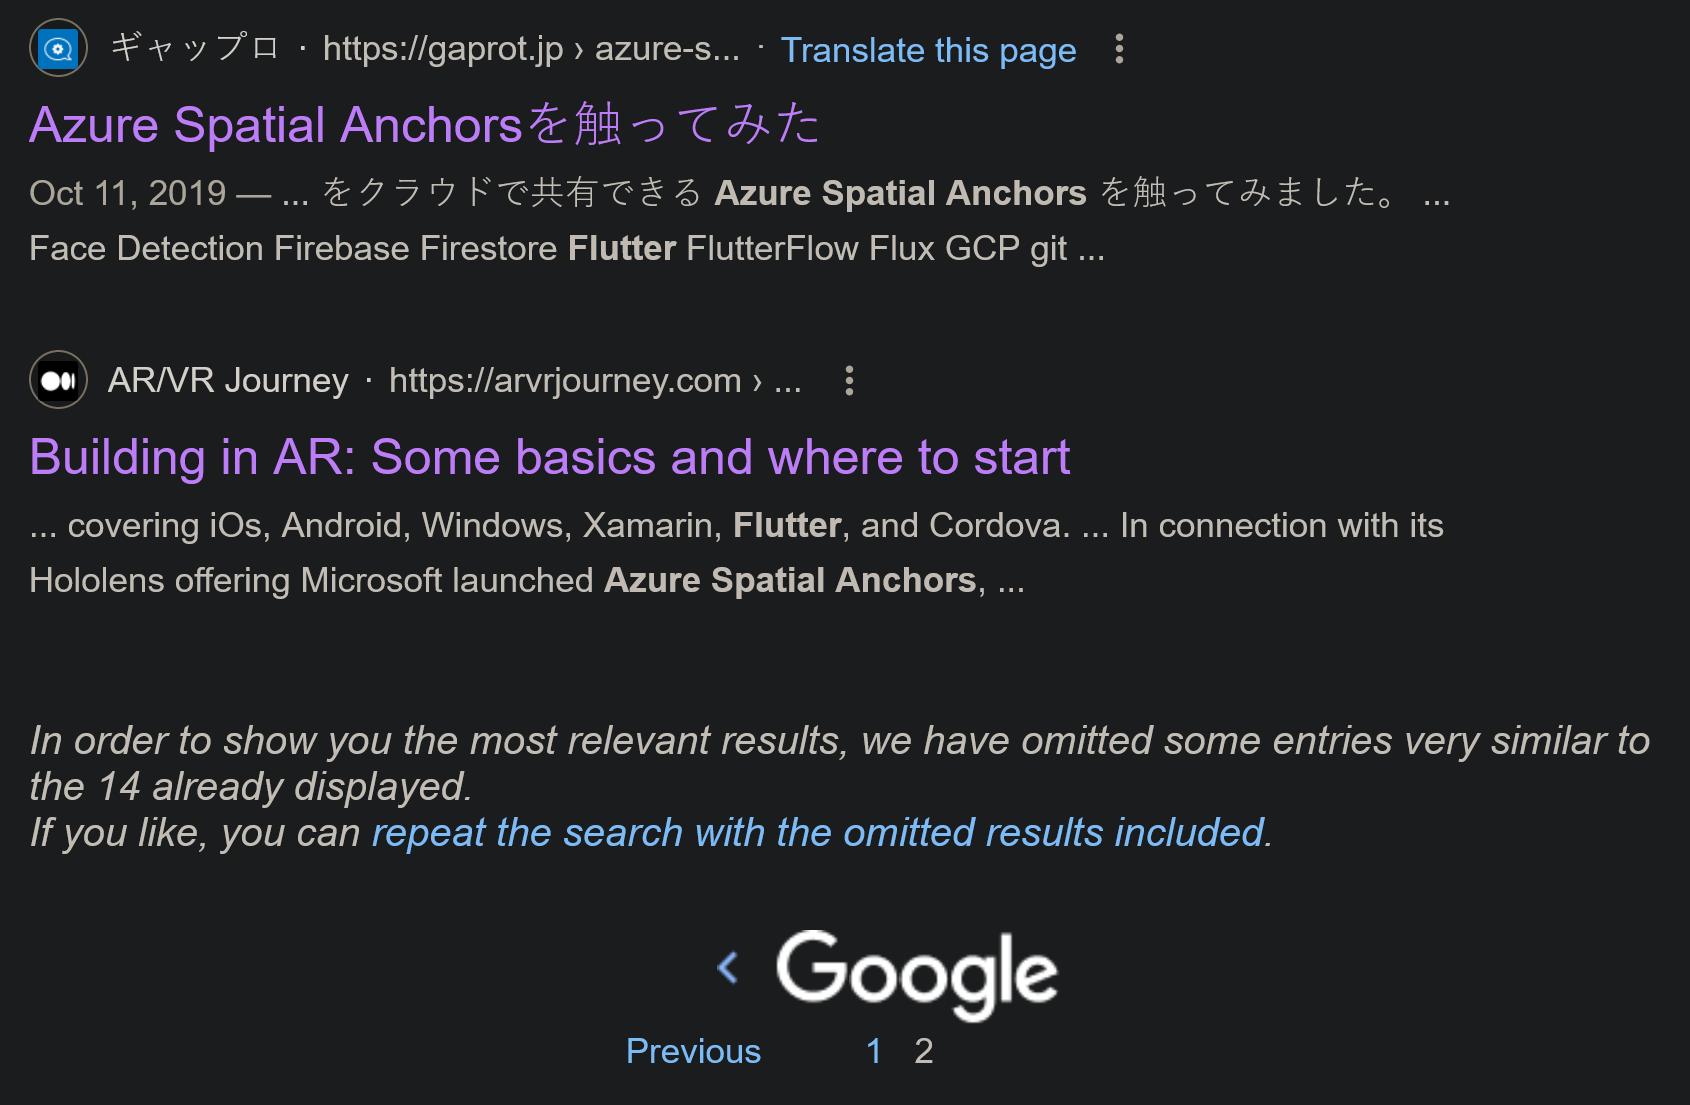
\includegraphics[width=.8\textwidth]{asa_flutter_search_today}
  \caption[Ricerca esatta Flutter e ASA 8 febbraio]{All'otto febbraio 2023 non si notano miglioramenti: solo 14 risultati rilevanti, alcuni in lingua giapponese, mostrano quando sia difficile trovare informazioni sull'argomento.}
  \label{fig:search2}
\end{figure}

Questa situazione ha significato dover risolvere tutti i problemi incontrati senza poter fare affidamento su alcun aiuto esterno e ha quindi esacerbato ulteriormente l'approccio \textit{trial-and-error} di cui si è parlato nella sezione \ref{sec:pianificazione}.

%************************************************************************************************************

\section{Analisi dei requisiti}
\label{sec:analisi_requisiti}
Di seguito sono riportati i requisti individuati nel piano di lavoro proposto e a seguito di opportuni confronti con il \textit{tutor} aziendale. Essi sono catalogati secondo la dicitura:
\begin{center}
    \textbf{R[Obbligatorietà][Tipologia][Codice]}
\end{center}
dove:
\begin{itemize}
    \item \textbf{Obbligatorietà}: specifica quanto un requisito sia vincolante per la riuscita del prodotto e può assumere i seguenti valori:
    \begin{itemize}
        \item \textbf{1: } Requisito obbligatorio;
        \item \textbf{2: } Requisito desiderabile ma non essenziale per il funzionamento;
        \item \textbf{3: } Requisito opzionale.
    \end{itemize}
    \item \textbf{Tipologia}: specifica la tipologia del requisito e può assumere i seguenti valori:
    \begin{itemize}
        \item \textbf{F: }\textit{funzionale,} determina una funzionalità necessaria all'applicazione;
        \item \textbf{V: }\textit{vincolo,} riguarda una caratteristica del prodotto decisa a monte.
    \end{itemize}
    \item \textbf{Codice}: identifica univocamente un requisito all'interno della sua tipologia (ovvero possono esistere due requisiti con lo stesso codice a patto che siano uno funzionale e uno di vincolo). Per i requisti subordinati si usa il "punto" come divisorio (\textit{ReqPadre, ReqPadre.Figlio1})
\end{itemize}

\subsection{Requisiti funzionali}
{
    \setlength{\freewidth}{\dimexpr\textwidth-10\tabcolsep}
    \renewcommand{\arraystretch}{1.5}
    \centering
    \setlength{\aboverulesep}{0pt}
    \setlength{\belowrulesep}{0pt}
    \rowcolors{2}{red!10}{white}
    \begin{longtable}{C{.15\freewidth} C{.965\freewidth}}
       \toprule
    \rowcolor{red}
    \textcolor{white}{\textbf{Codice}}&
    \textcolor{white}{\textbf{Descrizione}}\\
    \toprule
    \endhead

    R1F1 & Il \textit{plugin} deve rappresentare \textit{asset} tramite ancoraggio in realtà aumentata\\
    R1F2 & Il \textit{plugin} deve rappresentare \textit{ticket} tramite ancoraggio in realtà aumentata\\
    R1F3 & Il \textit{plugin} deve integrare gli ancoraggi tramite \asa{}\\
    R1F3.1 & Permettere aggiunta di \asa\\%C
    R1F3.2 & Permettere recupero e visualizzazione di \asa\\%R
    R2F3.3 & Permettere modifica di \asa\\%U
    R1F3.4 & Permettere eliminazione di \asa\\%D
    %API BACKEND
    R1F4 & Comunicare con le \api{} di Syn\\
    R1F4.1 & Ricevere \textit{asset} con ancoraggio associato\\
    R1F4.2 & Aggiungere \textit{asset} con ancoraggio associato\\
    R2F4.3 & Ricevere \textit{ticket} con ancoraggio associato\\
    R2F4.4 & Aggiungere \textit{ticket} con ancoraggio associato\\
    %UI FLUTTER
    R1F5 & Utente deve poter vedere quali \textit{asset} hanno ancoraggio associato\\
    R2F6 & Utente deve poter vedere quali \textit{ticket} hanno ancoraggio associato\\
    R1F7 & Utente deve poter raggiungere la vista in realtà aumentata dalla schermata degli \textit{asset}\\
    R1F8 & \textit{On-Tap} su una ancoraggio deve aprire una \textit{bottom sheet} contestuale\\
    R1F8.1 & \textit{Bottom sheet} deve presentare identificatore per \textit{asset} o \textit{ticket} associato all'ancoraggio\\
    R1F8.2 & \textit{Bottom sheet} associato a un \textit{asset} mostra \textit{ticket} aperti se presenti\\
    R1F8.3 & \textit{Bottom sheet} deve fornire \textit{Call-To-Action} per eliminare l'ancoraggio\\
    R1F8.4 & \textit{Bottom sheet} deve fornire \textit{Call-To-Action} per raggiungere pagina di dettaglio\\
    R1F9 & Le informazioni contestuali di un \textit{ticket} includono data e ora di creazione\\
    %UI AR
    R1F10 & Gli ancoraggi hanno rappresentazione visiva contestuale\\ 
    R1F11 & \textit{On-Tap} sullo spazio permette di creare una ancoraggio in posizione\\
    R1F11.1 & Ancoraggio posizionato nello spazio può essere salvato\\
    R1F11.2 & Ancoraggio posizionato nello spazio può essere eliminato\\
    R1F12 & Il salvataggio di un ancoraggio è disponibile solo quando è sicuro vada a buon fine\\
    R1F12.1 & Viene mostrato a schermo un feedback riguardo il livello di sicurezza raggiunto\\
    \bottomrule
    \rowcolor{white} 
    \caption{Tabella dei requisiti funzionali}
    \end{longtable}
}

\subsection{Requisiti di vincolo}
{
    \setlength{\freewidth}{\dimexpr\textwidth-10\tabcolsep}
    \renewcommand{\arraystretch}{1.5}
    \centering
    \setlength{\aboverulesep}{0pt}
    \setlength{\belowrulesep}{0pt}
    \rowcolors{2}{red!10}{white}
    \begin{longtable}{C{.15\freewidth} C{.965\freewidth}} 
       \toprule
    \rowcolor{red}
    \textcolor{white}{\textbf{Codice}}&
    \textcolor{white}{\textbf{Descrizione}}\\
    \toprule
    \endhead

    R1V1 & \textit{Framework} scelto funziona su Android\\
    R2V2 & \textit{Framework} scelto funziona su iOS\\
    R1V3 & \textit{Framework} scelto si integra con le \api{} di Syn\\
    R1V3.1 & \textit{Framework} ottiene con ancoraggio associato i dati degli \textit{asset}\\
    R1V3.2 & \textit{Framework} ottiene con ancoraggio associato i dati dei \textit{ticket}\\
    R1V4 & Il \textit{framework} scelto utilizza \asa\\
    R1V5 & La vista in realtà aumentata deve essere sviluppata in Flutter\\
    \bottomrule
    \rowcolor{white} 
    \caption{Tabella dei requisiti di vincolo}
    \end{longtable}
}

\subsection{Riepilogo requisiti}
Sono stati individuati un totale di 36 requisiti, 29 funzionali e 7 di vincolo, di seguito schematizzati:
{
    \setlength{\freewidth}{\dimexpr\textwidth-10\tabcolsep}
    \renewcommand{\arraystretch}{1.5}
    \centering
    \setlength{\aboverulesep}{0pt}
    \setlength{\belowrulesep}{0pt}
    \rowcolors{2}{red!10}{white}
    \begin{longtable}{C{.25\freewidth} C{.2\freewidth}} 
       \toprule
    \rowcolor{red}
    \textcolor{white}{\textbf{Obbligatorietà}}&
    \textcolor{white}{\textbf{Quantità}}\\
    \toprule
    \endhead

    Obbligatori & 31\\
    Desiderabili & 5\\
    \bottomrule
    \rowcolor{white} 
    \caption{Numero di requisiti per obbligatorietà}
    \label{tab:requisiti-obbligatorieta}
    \end{longtable}
}

{
    \setlength{\freewidth}{\dimexpr\textwidth-10\tabcolsep}
    \renewcommand{\arraystretch}{1.5}
    \centering
    \setlength{\aboverulesep}{0pt}
    \setlength{\belowrulesep}{0pt}
    \rowcolors{2}{red!10}{white}
    \begin{longtable}{C{.25\freewidth} C{.2\freewidth}} 
       \toprule
    \rowcolor{red}
    \textcolor{white}{\textbf{Tipologia}}&
    \textcolor{white}{\textbf{Quantità}}\\
    \toprule
    \endhead

    Funzionali & 29\\
    Di Vincolo & 7\\
    \bottomrule
    \rowcolor{white} 
    \caption{Numero di requisiti per tipologia}
    \label{tab:requisiti-tipolgia}
    \end{longtable}
}


%************************************************************************************************************

\section{Progettazione}
Tratterò la progettazione del sistema da due punti di vista: uno architetturale, che quindi pone l'accento su come il sistema sottostante svolga il lavoro di comunicazione con \asa{} e con le \api{} di Syn, e uno orientato invece all'aspetto grafico dell'applicazione, ovvero l'interfaccia utente.

\subsection{Architettura}
L'idea è di avere due sistemi comunicanti (gestiti con due diverse \textit{repository}): l'applicazione cliente MobileSYN che si interfaccia con Syn e il \textit{plugin} scelto che invece si occupa di gestire la parte in realtà aumentata e si interfaccia con \asa{}. \\
Bisogna fare chiarezza su un punto: Syn ha già in sistema degli \textit{asset} geolocalizzati tramite \asa{}, cioè quindi gli \textit{asset} sono legati a un ancoraggio del servizio di Microsoft, però questo è indipendente dal fatto che è sempre con \asa{} che implementiamo le componenti in realtà aumentata (in sostanza non è obbligatorio lavorare in \textit{augmented reality} per sfruttare gli ancoraggi di Azure). \\
Avremo quindi, a livello logico, MobileSYN che otterrà \textit{ticket} e \textit{asset} da Syn e poi li fornirà ad \aplug{} il quale si occuperà di mostrarli in realtà aumentata, fornendo anche la vista.

\begin{figure}[H]
  \centering
  %\includegraphics[height=5cm]{screen_mobilesyn}
  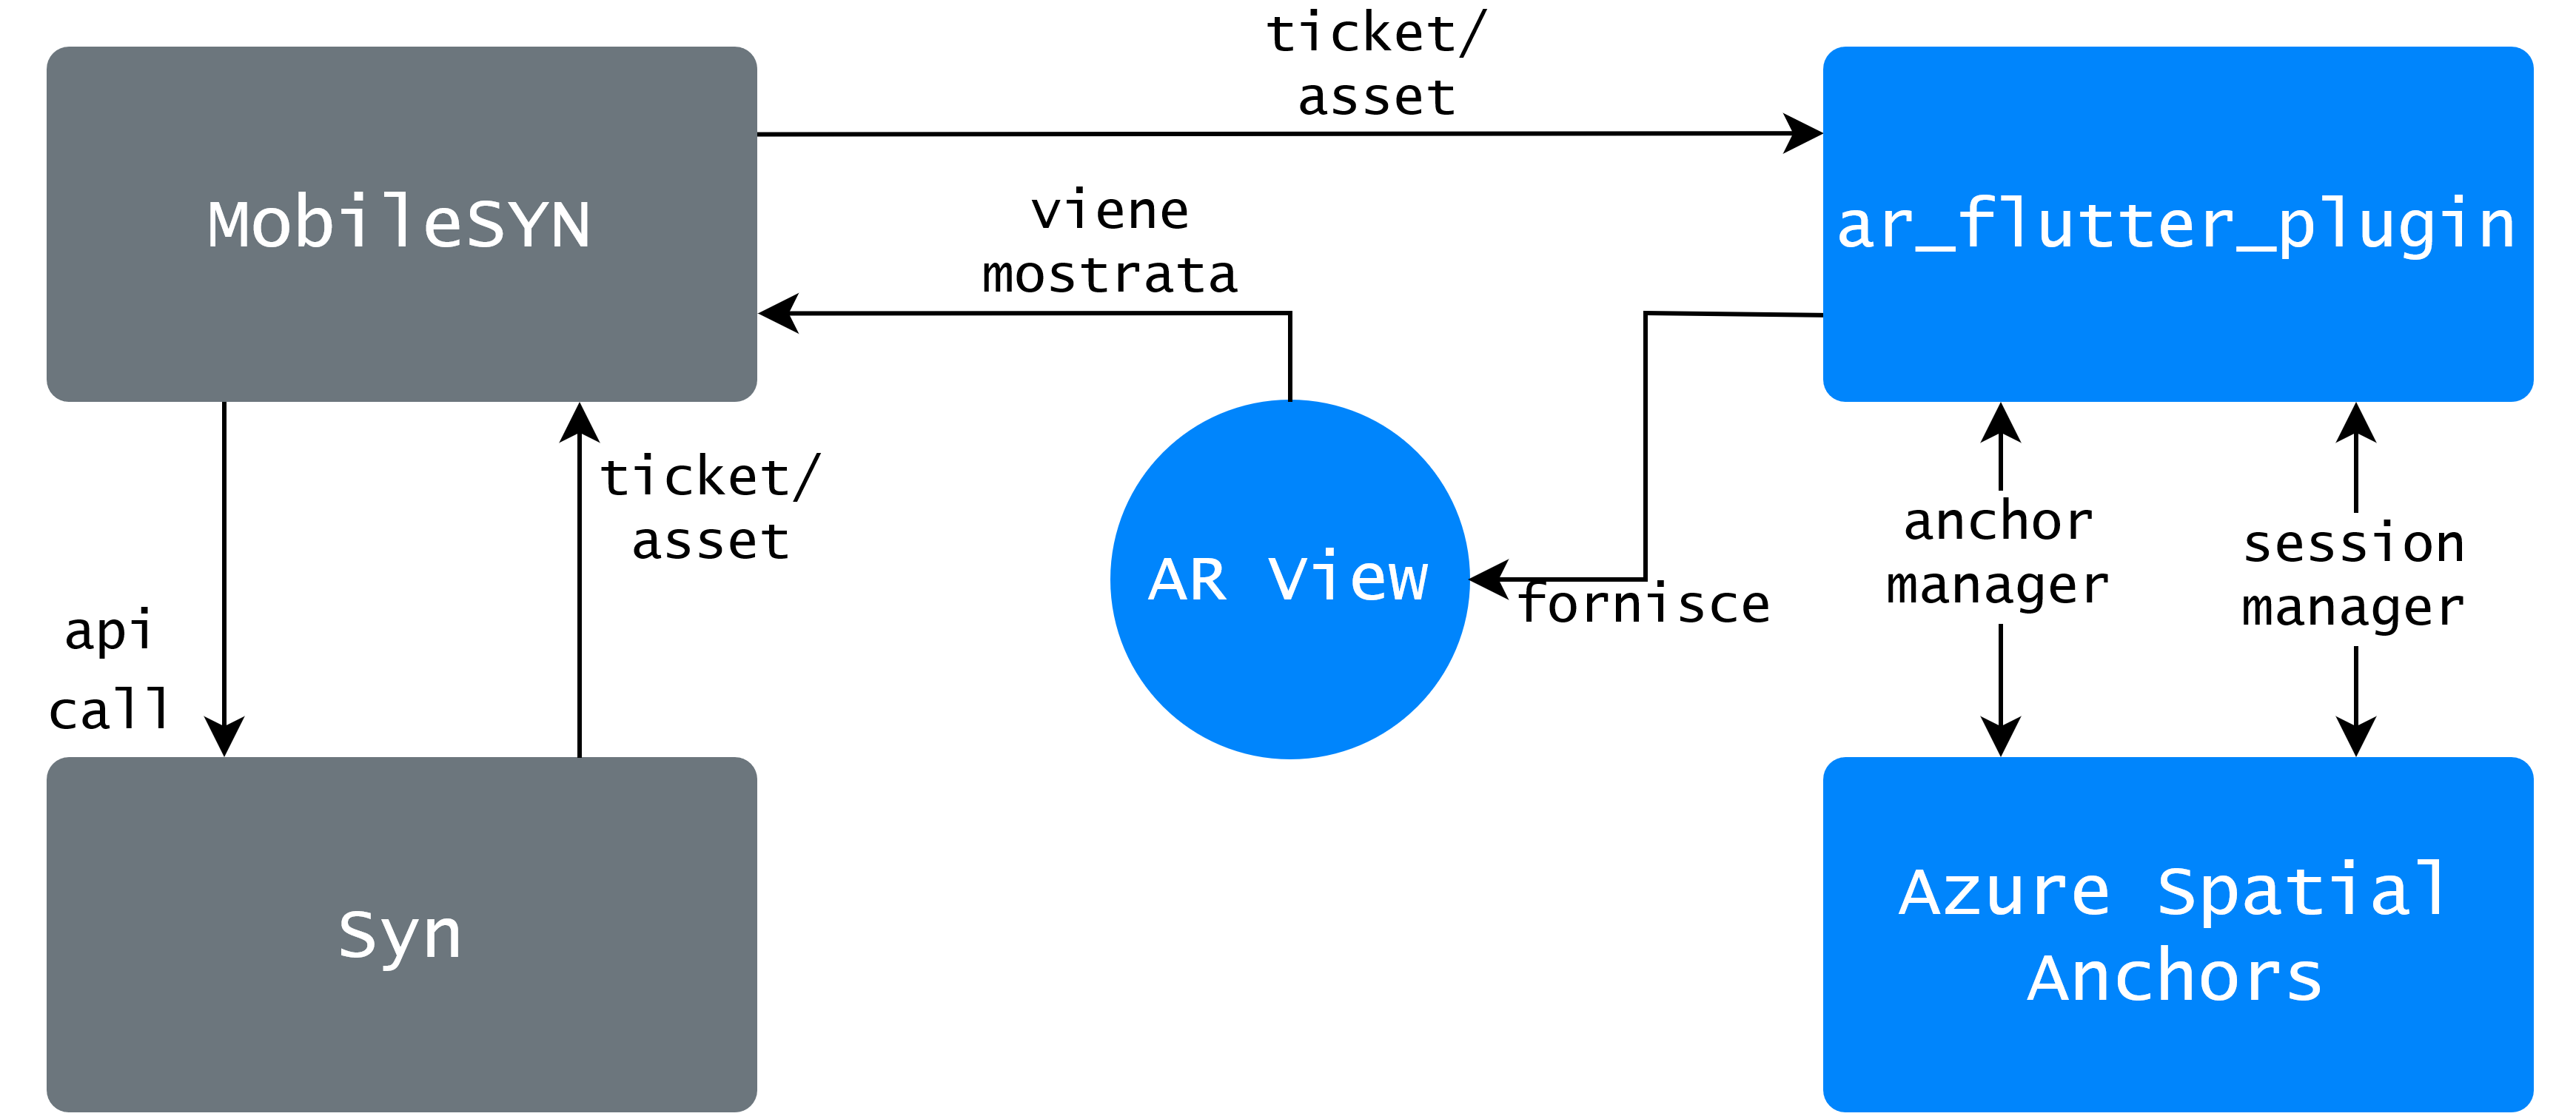
\includegraphics[width=\textwidth]{architettura}\hfill
  \caption[Architettura \textit{app}]{Rappresentazione dell'architettura dell'applicazione. MobileSYN fornisce \textit{ticket} e \textit{asset} a \aplug{} che di ritorno comunica con \asa{} per fornire all'applicazione cliente la vista in realtà aumentata.}
\end{figure}

\subsection{Interfaccia utente}
Mostro dei \textit{mockup} che danno un'idea di massima di come l'interfaccia utente dovrebbe presentarsi. Dai requisiti l'utente deve poter posizionare ancoraggi, caricarli sul \textit{cloud} quando sono stati ottenuti sufficienti dati spaziali e, all'\textit{on-tap} su una \textit{anchor}, deve vedere una \textit{bottom sheet} che gli presenti informazioni riguardo all'\textit{asset} collegato (ad esempio i \textit{ticket} aperti) e che gli permetta di raggiungere i dettagli dell'\textit{asset} o di eliminare l'\textit{anchor}.\\
Inoltre nella lista degli \textit{asset} devono essere presenti sia un'icona che identifichi quali hanno un ancoraggio associato posizionato in realtà aumentata e anche un bottone (in alto a destra in questo caso) che permetta di lanciare la vista.

\begin{figure}[H]
  \centering
  %\includegraphics[height=5cm]{screen_mobilesyn}
  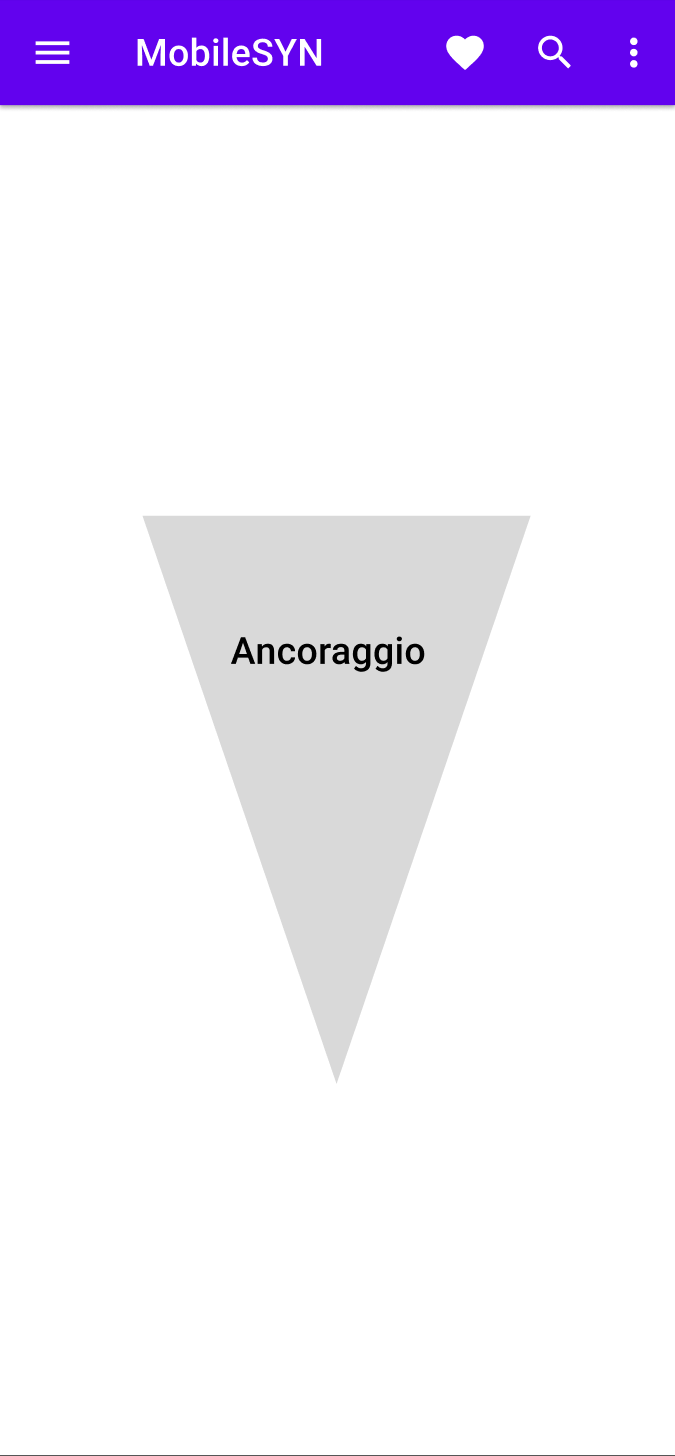
\includegraphics[width=.25\textwidth]{anchor_moc}\hfill
  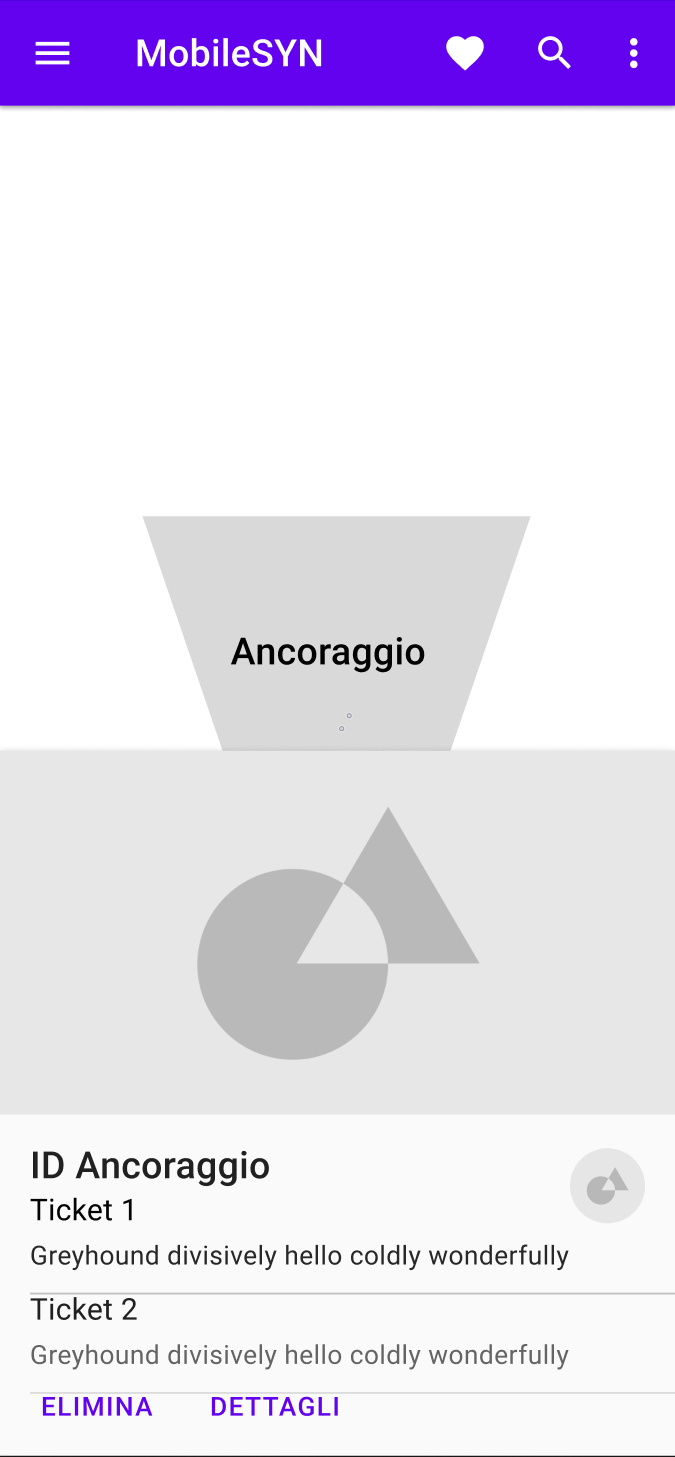
\includegraphics[width=.25\textwidth]{card_moc}\hfill
  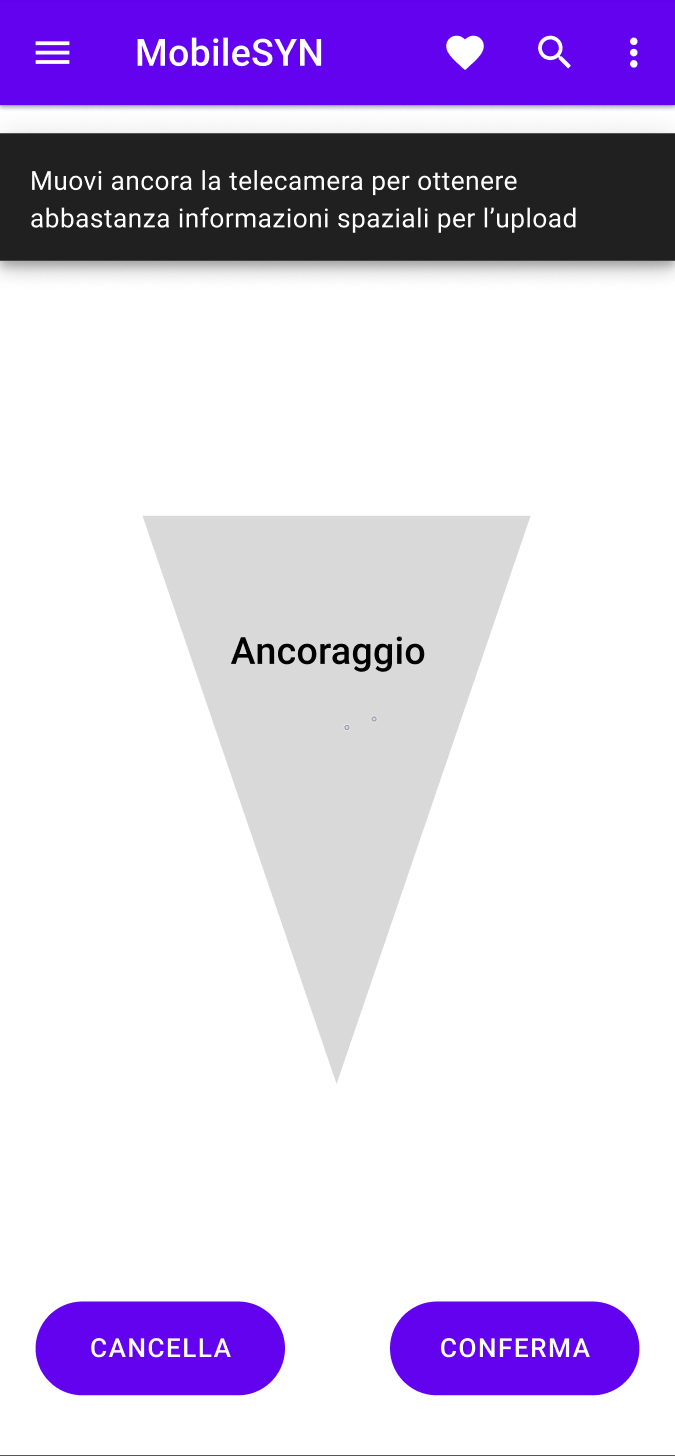
\includegraphics[width=.25\textwidth]{upload_moc}\hfill
  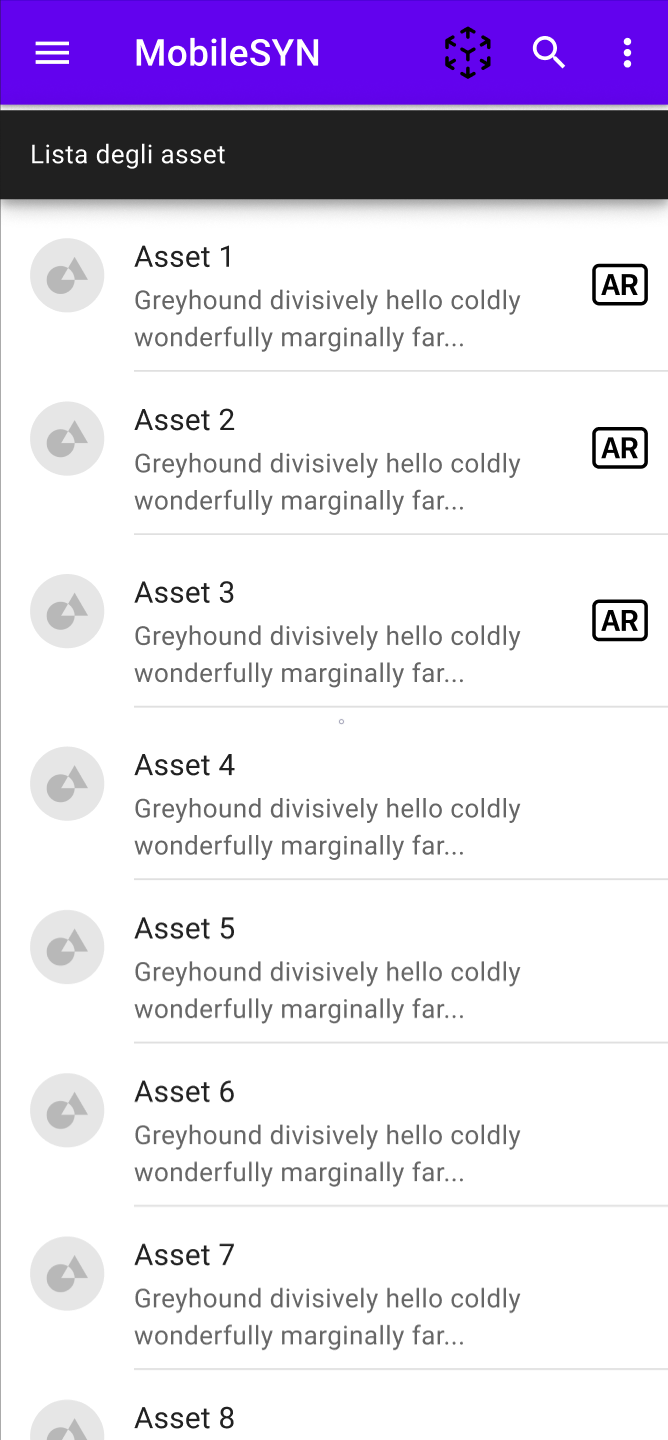
\includegraphics[width=.25\textwidth]{asset_list_moc}
  \caption[\textit{App mockup} ]{\textit{Mockup} per l'applicazione MobileSYN. In ordine: ancoraggio visto dalla telecamera, \textit{bottom sheet} contestuale che appare all'\textit{on-tap} sull'\textit{anchor}, schermata per caricare una \textit{anchor} in \textit{cloud}, lista degli \textit{asset}.}
\end{figure}

\section{Codifica}
Vediamo alcuni frammenti di codice che cercano di dare un'idea di massima di come, nel pratico, sono stati implementati i componenti in realtà aumentata. Partiamo quindi dalla parte in Dart, cioè quella comune. Il codice mostrato dovrà essere estremamente parziale, pena la creazione di un documento di diverse centinaia di pagine.\\
Il tutto è gestito con due \textit{repository} parallele: "mobilesyn" (che contiene il sorgente dell'applicazione vera e propria) e un \textit{fork} di "\aplug{}" alla quale sono state apportate le modifiche necessarie per interfacciarsi con SYN e le \asa{}. Partiamo dalla prima.\\
Vediamo un esempio di \textit{asset provider:}

\begin{lstlisting}[language=dart, label={lst:mobilesyn_asset_provider},firstnumber=1,caption={mobilesyn \textit{asset provider}}]
Future<void> fetchAssets(BusinessFunction? bf, GeoContainer? geoc) async 
  {
  debugPrint("FETCH-ASSETS");
  state = const AsyncValue.loading();
  try {
    final response = await read(synApiProvider).fetchAssets(
        count: 200, skip: 0, functionId: bf?.id, geocId: geoc?.id);
    state = AsyncValue.data(response);
  } catch (e) {
    debugPrint(e.toString());
    state = const AsyncValue.error('error_assets');
  }
}
\end{lstlisting} 

E di \textit{ticket provider}:

\begin{lstlisting}[language=dart, label={lst:mobilesyn_ticket_provider}, firstnumber=1,caption={mobilesyn \textit{ticket provider}}]
Future<void> fetchTickets(String flowId, bool closed) async {
  debugPrint("FETCH-TICKETS");
  state = const AsyncValue.loading();
  try {
    var tpl = read(ticketsfiltersProvider).template;
    var since = read(ticketsfiltersProvider).since;
    var till = read(ticketsfiltersProvider).till;
    var geoc = read(selectedGeocP);
    final tickets = await read(synApiProvider).fetchTickets(
        skip: 0,
        count: 100,
        flowId: flowId,
        closed: closed,
        tplId: tpl?.id,
        since: closed ? since : null,
        till: closed ? till : null,
        geocId: geoc?.id);
    final List<TicketAssetInfo> temp =
        tickets.map((t) => t.asset).whereType<TicketAssetInfo>()
                                   .toList();
    final strings = temp.map((e) => e.toJson()).toList().toSet()
                                     .toList();
    final List<TicketAssetInfo> assets =
        strings.map((e) => TicketAssetInfo.fromJson(e)).toList();
    final FeatureList featured = FeatureList.fromTicketList(tickets);
    state = AsyncValue.data(TicketStateModel(
        tickets: tickets, assets: assets, featured: featured));
  } catch (e) {
    debugPrint(e.toString());
    state = const AsyncValue.error('error_asset_tickets');
  }
}
\end{lstlisting} 

Notiamo, per entrambi, l'uso di un \verb+Future+. Nella pagina che si occupa di mostrare i dettagli di un \textit{asset} abbiamo una funzione specifica per ottenere i \textit{ticket} a esso associati:

\begin{lstlisting}[language=dart, label={lst:mobilesyn_asset_ticket_provider}, firstnumber=1,caption={mobilesyn \textit{asset ticket provider}}]
Future<void> fetchAssetTickets() async {
  debugPrint('FETCH ASSET TICKETS - ${asset.cod}');
  try {
    loadingTickets.value = true;
    errorTickets.value = false;
    final response = await ref
        .read(synApiProvider)
        .fetchTickets(skip: 0, count: 3, assetId: asset.id!);
    loadingTickets.value = false;
    errorTickets.value = false;
    tickets.value = response;
  } catch (e) {
    debugPrint(e.toString());
    loadingTickets.value = false;
    errorTickets.value = true;
    tickets.value = [];
  }
}
\end{lstlisting} 



Per quanto riguarda invece i \textit{manager} delle componenti in realtà aumenta essi vengono presi da \aplug{}:

\begin{lstlisting}[language=dart, label={lst:mobilesyn_managers}, firstnumber=1,caption={mobilesyn \textit{managers}}]
import 'package:ar_flutter_plugin/managers/ar_anchor_manager.dart';
import 'package:ar_flutter_plugin/managers/ar_session_manager.dart';

class ManagementArView extends HookConsumerWidget {
  const ManagementArView({Key? key}) : super(key: key);

  @override
  Widget build(BuildContext context, WidgetRef ref) {
    final arSessionManager = useState<ARSessionManager?>(null);
    final arAnchorManager = useState<ARAnchorManager?>(null);
\end{lstlisting} 

E sono state costruite diverse funzioni di utilità, ad esempio il seguente codice viene chiamato alla creazione della vista:

\begin{lstlisting}[language=dart, label={lst:mobilesyn_onARViewCreated}, firstnumber=1,caption={mobilesyn \textit{on ar view created}}]
void onARViewCreated(
  ARSessionManager _arSessionManager, ARAnchorManager _arAnchorManager) {
arSessionManager.value = _arSessionManager;
arAnchorManager.value = _arAnchorManager;
arAnchorManager.value!.onAssetTap = onAssetTap;
arAnchorManager.value!.onTicketTap = onTicketTap;
arViewInitialized.value = true;
}
\end{lstlisting} 

{
    \setlength{\freewidth}{\dimexpr\textwidth-10\tabcolsep}
    \renewcommand{\arraystretch}{1.5}
    \centering
    \setlength{\aboverulesep}{0pt}
    \setlength{\belowrulesep}{0pt}
    \rowcolors{2}{red!10}{white}
    \begin{longtable}{C{.15\freewidth} C{.965\freewidth}}
       \toprule
    \rowcolor{red}
    \textcolor{white}{\textbf{Codice}}&
    \textcolor{white}{\textbf{Descrizione}}\\
    \toprule
    \endhead

    R1V3 & \textit{Framework} scelto si integra con le \api{} di Syn\\
    R1V3.1 & \textit{Framework} ottiene con ancoraggio associato i dati degli \textit{asset}\\
    R1V3.2 & \textit{Framework} ottiene con ancoraggio associato i dati dei \textit{ticket}\\ 
    R1F4 & Comunicare con le \api{} di Syn\\
    R1F4.1 & Ricevere \textit{asset} con ancoraggio associato\\
    R1F4.2 & Aggiungere \textit{asset} con ancoraggio associato\\
    R2F4.3 & Ricevere \textit{ticket} con ancoraggio associato\\
    R2F4.4 & Aggiungere \textit{ticket} con ancoraggio associato\\
  
    \bottomrule
    \rowcolor{white} 
    \caption{Requisiti soddisfatti nei frammenti: \ref{lst:mobilesyn_asset_provider}, \ref{lst:mobilesyn_ticket_provider}, \ref{lst:mobilesyn_asset_ticket_provider}, \ref{lst:mobilesyn_managers}, \ref{lst:mobilesyn_onARViewCreated}.}
    \end{longtable}
}

Passiamo quindi a vedere alcuni frammenti dei \textit{manager} di \aplug{}.
Nel \textit{manager} per gli ancoraggi vediamo i metodi per creazione ed eliminazione di \textit{anchor} localmente e per \textit{upload} ed eliminazione di ancoraggi in \textit{cloud} (si noti che tutti i metodi usano i \textit{method channels}): 

\begin{lstlisting}[language=dart, label={lst:arplug_manager}, firstnumber=1,caption={\aplug{} \textit{create, delete, ulpoad, delete cloud anchor} tramite \textit{method channel}}]
Future<void> createAnchor(
    {required Matrix4 transformation,
    required Map<String, dynamic> info}) async {
  return await _channel.invokeMethod<void>('createAnchor', {
    "transformation": MatrixConverter().toJson(transformation),
    "info": info
  });
}

/// Remove given anchor and all its children from the AR Scene
Future<void> deleteAnchor({required String anchorId}) async {
  return await _channel.invokeMethod<void>('deleteAnchor',
                                          {'id': anchorId});
}

/// Upload the latest added Anchor to the ASA Cloud
Future<String?> uploadAnchor() async {
  try {
    return await _channel.invokeMethod<String?>('uploadAnchor');
  } on PlatformException catch (_) {
    return null;
  }
}

/// Delete the given anchor from the ASA Cloud and the AR Scene
Future<bool?> deleteCloudAnchor({required String anchorId}) async {
  try {
    return await _channel
        .invokeMethod<bool?>('deleteCloudAnchor', {'id': anchorId});
  } on PlatformException catch (_) {
    return null;
  }
}
\end{lstlisting} 

Queste chiamate in Android sono implementati tramite chiamate Java innestate in Kotlin:

\begin{lstlisting}[language=Kotlin, label={lst:android_channels}, firstnumber=1,caption={Android chiamate dei \textit{method channel} per effettuare \textit{create, delete, ulpoad, delete cloud anchor} tramite \textit{method channel}}]
private val onAnchorMethodCall =
MethodChannel.MethodCallHandler { call, result ->
    when (call.method) {
        "createAnchor" -> {
            val dictInfo = call.argument("info") as HashMap<String,
                                                            Any>?
            val transform = call.argument("transformation") 
                                 as ArrayList<Double>?
            createAnchor(transform!!, AnchorInfo(dictInfo!!))
            result.success(null)
        }
        "uploadAnchor" -> {
            uploadAnchor(result)
        }
        "deleteAnchor" -> {
            val infoId = call.argument("id") as String?
            deleteAnchor(infoId!!)
            result.success(null)
        }
        "deleteCloudAnchor" -> {
            val infoId = call.argument("id") as String?
            deleteCloudAnchor(infoId!!, result)
        }
        else -> {
            Log.d(TAG, call.method + "not supported on anchorManager")
        }
    }
}
\end{lstlisting}

Mentre per quanto riguarda iOS sono implementate in Swift:

\begin{lstlisting}[language=swift, label={lst:ios_channels}, firstnumber=1,caption={iOS chiamate dei \textit{method channel} per effettuare \textit{create, delete, ulpoad, delete cloud anchor}}]
func onAnchorMethodCalled(_ call: FlutterMethodCall, _ result: 
                                      @escaping FlutterResult) {
  let arguments = call.arguments as? [String: Any]
  NSLog("IosARView: onAnchorMethodCalled \(call.method)")
  switch call.method {
      case "createAnchor":
          let dictInfo = arguments?["info"] as! [String: Any]
          let transform = arguments?["transformation"] as! [NSNumber]
          createAnchor(transform: transform, info: 
                                             AnchorInfo(val: dictInfo))
          result(nil)
      case "uploadAnchor":
          uploadAnchor(result: result)
      case "deleteAnchor":
          let infoId = arguments!["id"] as! String
          deleteAnchor(infoId: infoId)
          result(nil)
      case "deleteCloudAnchor":
          let infoId = arguments!["id"] as! String
          deleteCloudAnchor(infoId: infoId, result: result)
      default:
          result(FlutterMethodNotImplemented)
  }
}
\end{lstlisting}

Vediamo un piccolo esempio di come vengono implementate, in Android, le \asa{}. Non porteremo in questo caso l'esempio speculare di iOS in quanto poco interessante: come si vede dai frammenti di codice precedenti le differenze sono più tecniche che macroscopiche.\\
Vediamo l'eliminazione di un ancoraggio salvato in \textit{cloud}, riprendendo il codice in \ref{lst:android_channels} guardiamo il flusso che provoca la chiamata \verb+"deleteCloudAnchor"+:

\begin{lstlisting}[language=dart, label={lst:asa_android_call}, firstnumber=1,caption={Eliminazione \textit{cloud anchor} lato Android, chiamata}]
private fun deleteCloudAnchor(infoId: String,
                              result: MethodChannel.Result) {
  Log.d(TAG, "removeCloudAnchor $infoId")
  val visual = anchorVisuals[infoId]
  if (visual?.cloudAnchor != null) {
      azureSpatialAnchorsManager!!.
      deleteAnchorAsync(visual.cloudAnchor!!)

  //la funzione prosegue ma non ci interessa per questa dimostrazione
\end{lstlisting}

Vediamo che è stato chiamato in causa il \textit{manager} per le \asa{}, seguiamo quindi il flusso:

\begin{lstlisting}[language=dart, label={lst:asa_manager_delete}, firstnumber=1,caption={Eliminazione \textit{cloud anchor} lato Android, chiamata}]
internal class AzureSpatialAnchorsManager(arCoreSession: Session?, 
                                          apiKey: String, apiId: String) {
  private val executorService: ExecutorService = Executors.
                                                 newFixedThreadPool(2)
  var isRunning = false
  private val spatialAnchorsSession: CloudSpatialAnchorSession
  // Set this string to the account ID provided 
  //for the Azure Spatial Anchors account resource.
  private val SpatialAnchorsAccountId = apiId

  // Set this string to the account key provided 
  //for the Azure Spatial Anchors account resource.
  private val SpatialAnchorsAccountKey = apiKey

  //ora viene chiamata l'effettiva eliminazione
  fun deleteAnchorAsync(anchor: CloudSpatialAnchor?): 
                                CompletableFuture<*> {
        return toEmptyCompletableFuture(spatialAnchorsSession.
                                        deleteAnchorAsync(anchor))
  }
\end{lstlisting}

Grazie al codice appena visto possiamo notare che l'applicazione comunica con le \api{} di SYN per ottenere \textit{ticket} e \textit{asset}, e che ottiene gli ancoraggi e che questi ancoraggi sono gestiti tramite \asa{}. Inoltre abbiamo visto che tutto questo è stato implementato sia in Android che in iOS e che la vista è scritta in Flutter.

{
    \setlength{\freewidth}{\dimexpr\textwidth-10\tabcolsep}
    \renewcommand{\arraystretch}{1.5}
    \centering
    \setlength{\aboverulesep}{0pt}
    \setlength{\belowrulesep}{0pt}
    \rowcolors{2}{red!10}{white}
    \begin{longtable}{C{.15\freewidth} C{.965\freewidth}}
       \toprule
    \rowcolor{red}
    \textcolor{white}{\textbf{Codice}}&
    \textcolor{white}{\textbf{Descrizione}}\\
    \toprule
    \endhead

    R1V1 & \textit{Framework} scelto funziona su Android\\
    R2V2 & \textit{Framework} scelto funziona su iOS\\
    R1V4 & Il \textit{framework} scelto utilizza \asa\\
    R1F3 & Il \textit{plugin} deve integrare gli ancoraggi tramite \asa{}\\
    R1F3.1 & Permettere aggiunta di \asa\\%C
    R1F3.2 & Permettere recupero e visualizzazione di \asa\\%R
    R2F3.3 & Permettere modifica di \asa\\%U
    R1F3.4 & Permettere eliminazione di \asa\\%D
  
    \bottomrule
    \rowcolor{white} 
    \caption{Requisiti soddisfatti nei frammenti: \ref{lst:arplug_manager}, \ref{lst:android_channels}, \ref{lst:ios_channels}, \ref{lst:asa_android_call}, \ref{lst:asa_manager_delete}.}
    \end{longtable}
}

Vediamo infine una piccola parte del codice che si occupa di creare l'effettiva interfaccia utente della vista in realtà aumentata:

\begin{lstlisting}[language=dart, label={lst:ar_view}, firstnumber=1,caption={Frammento di codice per vista in realtà aumenta in Dart}]
/// Android-specific implementation of [PlatformARView]
class AndroidARView implements PlatformARView {
  late BuildContext? _context;
  late ARViewCreatedCallback? _arViewCreatedCallback;
  
  @override
  void onPlatformViewCreated(int id) {
    print("Android platform view created!");
    createManagers(id, _context, _arViewCreatedCallback);
  }
  
  @override
  Widget build(
      {BuildContext? context,
      ARViewCreatedCallback? arViewCreatedCallback,
      String? apiKey,
      String? apiId,
      List<Map<String, dynamic>>? assets,
      List<Map<String, dynamic>>? tickets}) {
      \\altro codice
      }
  \\altro codice
}


/// iOS-specific implementation of [PlatformARView]
class IosARView implements PlatformARView {
  BuildContext? _context;
  ARViewCreatedCallback? _arViewCreatedCallback;

  @override
  void onPlatformViewCreated(int id) {
    print("iOS platform view created!");
    createManagers(id, _context, _arViewCreatedCallback);
  }

  @override
  Widget build(
      {BuildContext? context,
      ARViewCreatedCallback? arViewCreatedCallback,
      String? apiKey,
      String? apiId,
      List<Map<String, dynamic>>? assets,
      List<Map<String, dynamic>>? tickets}) {
      \\altro codice
      }
  \\altro codice
}
\end{lstlisting}

{
    \setlength{\freewidth}{\dimexpr\textwidth-10\tabcolsep}
    \renewcommand{\arraystretch}{1.5}
    \centering
    \setlength{\aboverulesep}{0pt}
    \setlength{\belowrulesep}{0pt}
    \rowcolors{2}{red!10}{white}
    \begin{longtable}{C{.15\freewidth} C{.965\freewidth}}
       \toprule
    \rowcolor{red}
    \textcolor{white}{\textbf{Codice}}&
    \textcolor{white}{\textbf{Descrizione}}\\
    \toprule
    \endhead

    R1V5 & La vista in realtà aumentata deve essere sviluppata in Flutter\\
  
    \bottomrule
    \rowcolor{white} 
    \caption{Requisiti soddisfatti nel frammento: \ref{lst:ar_view}}
    \end{longtable}
}

\section{Verifica e validazione}

\section{Copertura requisti}
L'unico requisito rimasto insoddisfatto è il seguente:
{
    \setlength{\freewidth}{\dimexpr\textwidth-10\tabcolsep}
    \renewcommand{\arraystretch}{1.5}
    \centering
    \setlength{\aboverulesep}{0pt}
    \setlength{\belowrulesep}{0pt}
    \rowcolors{2}{red!10}{white}
    \begin{longtable}{C{.15\freewidth} C{.965\freewidth}} 
       \toprule
    \rowcolor{red}
    \textcolor{white}{\textbf{Codice}}&
    \textcolor{white}{\textbf{Descrizione}}\\
    \toprule
    \endhead

    R2F6 & Utente deve poter vedere quali \textit{ticket} hanno ancoraggio associato\\

    \bottomrule
    \rowcolor{white} 
    \caption{Requisiti non soddisfatti}
    \end{longtable}
}

Portando quindi la copertura totale dei requisiti a un livello più che soddisfacente.\\
Vediamo quindi una sintesi, in tabella singola, dei requisti soddisfatti e dove vederne la dimostrazione (figure o frammenti di codice).

{
    \setlength{\freewidth}{\dimexpr\textwidth-10\tabcolsep}
    \renewcommand{\arraystretch}{1.5}
    \centering
    \setlength{\aboverulesep}{0pt}
    \setlength{\belowrulesep}{0pt}
    \rowcolors{2}{red!10}{white}
    \begin{longtable}{C{.3\freewidth} C{.4\freewidth}} 
       \toprule
    \rowcolor{red}
    \textcolor{white}{\textbf{Codice requisito}}&
    \textcolor{white}{\textbf{Dove trovarne il soddisfacimento}}\\
    \toprule
    \endhead

    R1V1 &\ref{lst:arplug_manager}, \ref{lst:android_channels}, \ref{lst:ios_channels}, \ref{lst:asa_android_call}, \ref{lst:asa_manager_delete}\\
    R2V2 &\ref{lst:arplug_manager}, \ref{lst:android_channels}, \ref{lst:ios_channels}, \ref{lst:asa_android_call}, \ref{lst:asa_manager_delete}\\
    R1V3 &\ref{lst:mobilesyn_asset_provider}, \ref{lst:mobilesyn_ticket_provider}, \ref{lst:mobilesyn_asset_ticket_provider}, \ref{lst:mobilesyn_managers}, \ref{lst:mobilesyn_onARViewCreated}\\
    R1V3.1 &\ref{lst:mobilesyn_asset_provider}, \ref{lst:mobilesyn_ticket_provider}, \ref{lst:mobilesyn_asset_ticket_provider}, \ref{lst:mobilesyn_managers}, \ref{lst:mobilesyn_onARViewCreated}\\
    R1V3.2 &\ref{lst:mobilesyn_asset_provider}, \ref{lst:mobilesyn_ticket_provider}, \ref{lst:mobilesyn_asset_ticket_provider}, \ref{lst:mobilesyn_managers}, \ref{lst:mobilesyn_onARViewCreated}\\
    R1V4 &\ref{lst:arplug_manager}, \ref{lst:android_channels}, \ref{lst:ios_channels}, \ref{lst:asa_android_call}, \ref{lst:asa_manager_delete}\\
    R1V5 &\ref{lst:ar_view}\\

    R1F1 & \ref{fig:place_asset}\\
    R1F2 & \ref{fig:ticket_ar}\\
    R1F3 &\ref{lst:arplug_manager}, \ref{lst:android_channels}, \ref{lst:ios_channels}, \ref{lst:asa_android_call}, \ref{lst:asa_manager_delete}\\
    R1F3.1 &\ref{lst:arplug_manager}, \ref{lst:android_channels}, \ref{lst:ios_channels}, \ref{lst:asa_android_call}, \ref{lst:asa_manager_delete}\\%C
    R1F3.2 &\ref{lst:arplug_manager}, \ref{lst:android_channels}, \ref{lst:ios_channels}, \ref{lst:asa_android_call}, \ref{lst:asa_manager_delete}\\%R
    R2F3.3 &\ref{lst:arplug_manager}, \ref{lst:android_channels}, \ref{lst:ios_channels}, \ref{lst:asa_android_call}, \ref{lst:asa_manager_delete}\\%U
    R1F3.4 &\ref{lst:arplug_manager}, \ref{lst:android_channels}, \ref{lst:ios_channels}, \ref{lst:asa_android_call}, \ref{lst:asa_manager_delete}\\%D
    %API BACKEND
    R1F4 &\ref{lst:mobilesyn_asset_provider}, \ref{lst:mobilesyn_ticket_provider}, \ref{lst:mobilesyn_asset_ticket_provider}, \ref{lst:mobilesyn_managers}, \ref{lst:mobilesyn_onARViewCreated} \\
    R1F4.1 &\ref{lst:mobilesyn_asset_provider}, \ref{lst:mobilesyn_ticket_provider}, \ref{lst:mobilesyn_asset_ticket_provider}, \ref{lst:mobilesyn_managers}, \ref{lst:mobilesyn_onARViewCreated}\\
    R1F4.2 &\ref{lst:mobilesyn_asset_provider}, \ref{lst:mobilesyn_ticket_provider}, \ref{lst:mobilesyn_asset_ticket_provider}, \ref{lst:mobilesyn_managers}, \ref{lst:mobilesyn_onARViewCreated}\\
    R2F4.3 &\ref{lst:mobilesyn_asset_provider}, \ref{lst:mobilesyn_ticket_provider}, \ref{lst:mobilesyn_asset_ticket_provider}, \ref{lst:mobilesyn_managers}, \ref{lst:mobilesyn_onARViewCreated}\\
    R2F4.4 &\ref{lst:mobilesyn_asset_provider}, \ref{lst:mobilesyn_ticket_provider}, \ref{lst:mobilesyn_asset_ticket_provider}, \ref{lst:mobilesyn_managers}, \ref{lst:mobilesyn_onARViewCreated}\\
    %UI FLUTTER
    R1F5 & \ref{fig:asset_list}\\
    R2F6 & Non soddisfatto \\
    R1F7 & \ref{fig:asset_list}\\
    R1F8 & \ref{fig:asset_list}\\
    R1F8.1 & \ref{fig:asset_list}\\
    R1F8.2 & \ref{fig:asset_list}\\
    R1F8.3 &\ref{fig:asset_list}\\
    R1F8.4 & \ref{fig:asset_list}\\
    R1F9 & \ref{fig:ticket_ar}\\
    %UI AR
    R1F10 &\ref{fig:ticket_ar}\\ 
    R1F11 &\ref{fig:place_asset} \\
    R1F11.1 & \ref{fig:place_asset}\\
    R1F11.2 & \ref{fig:place_asset}\\
    R1F12 & \ref{fig:place_asset}\\
    R1F12.1 & \ref{fig:place_asset}\\
    
    \bottomrule
    \rowcolor{white} 
    \caption[Tabella requisiti - chi li soddisfa]{Tabella che mette in relazione i requisiti e dove si vede il loro soddisfacimento.}
    \end{longtable}
}

\section{Risultati raggiunti}
In quest'ultima sezione vediamo il risultato finale del lavoro di stage, partendo col mettere in relazione i requisiti individuati nella sezione \ref{sec:analisi_requisiti} con le \textit{screenshot} di MobileSYN.\\
Le seguenti immagini mostrano il progresso in vista in realtà aumentata che porta a creare un ancoraggio relativo all'\textit{asset} "IT-TESTP-ELight0324" (privo di eventi o \textit{ticket} correlati), per poi caricarlo in \textit{cloud} e, successivamente a chiusura e riapertura dell'applicazione, ritrovarlo in posizione (si noti che è leggermente arretrato).\\
Inoltre nella prima immagine, viene anche mostrato il livello di progressione di \textit{scan} dell'ambiente, necessario a caricare correttamente un ancoraggio.

\begin{figure}[H]
  \centering
  %\includegraphics[height=5cm]{screen_mobilesyn}
  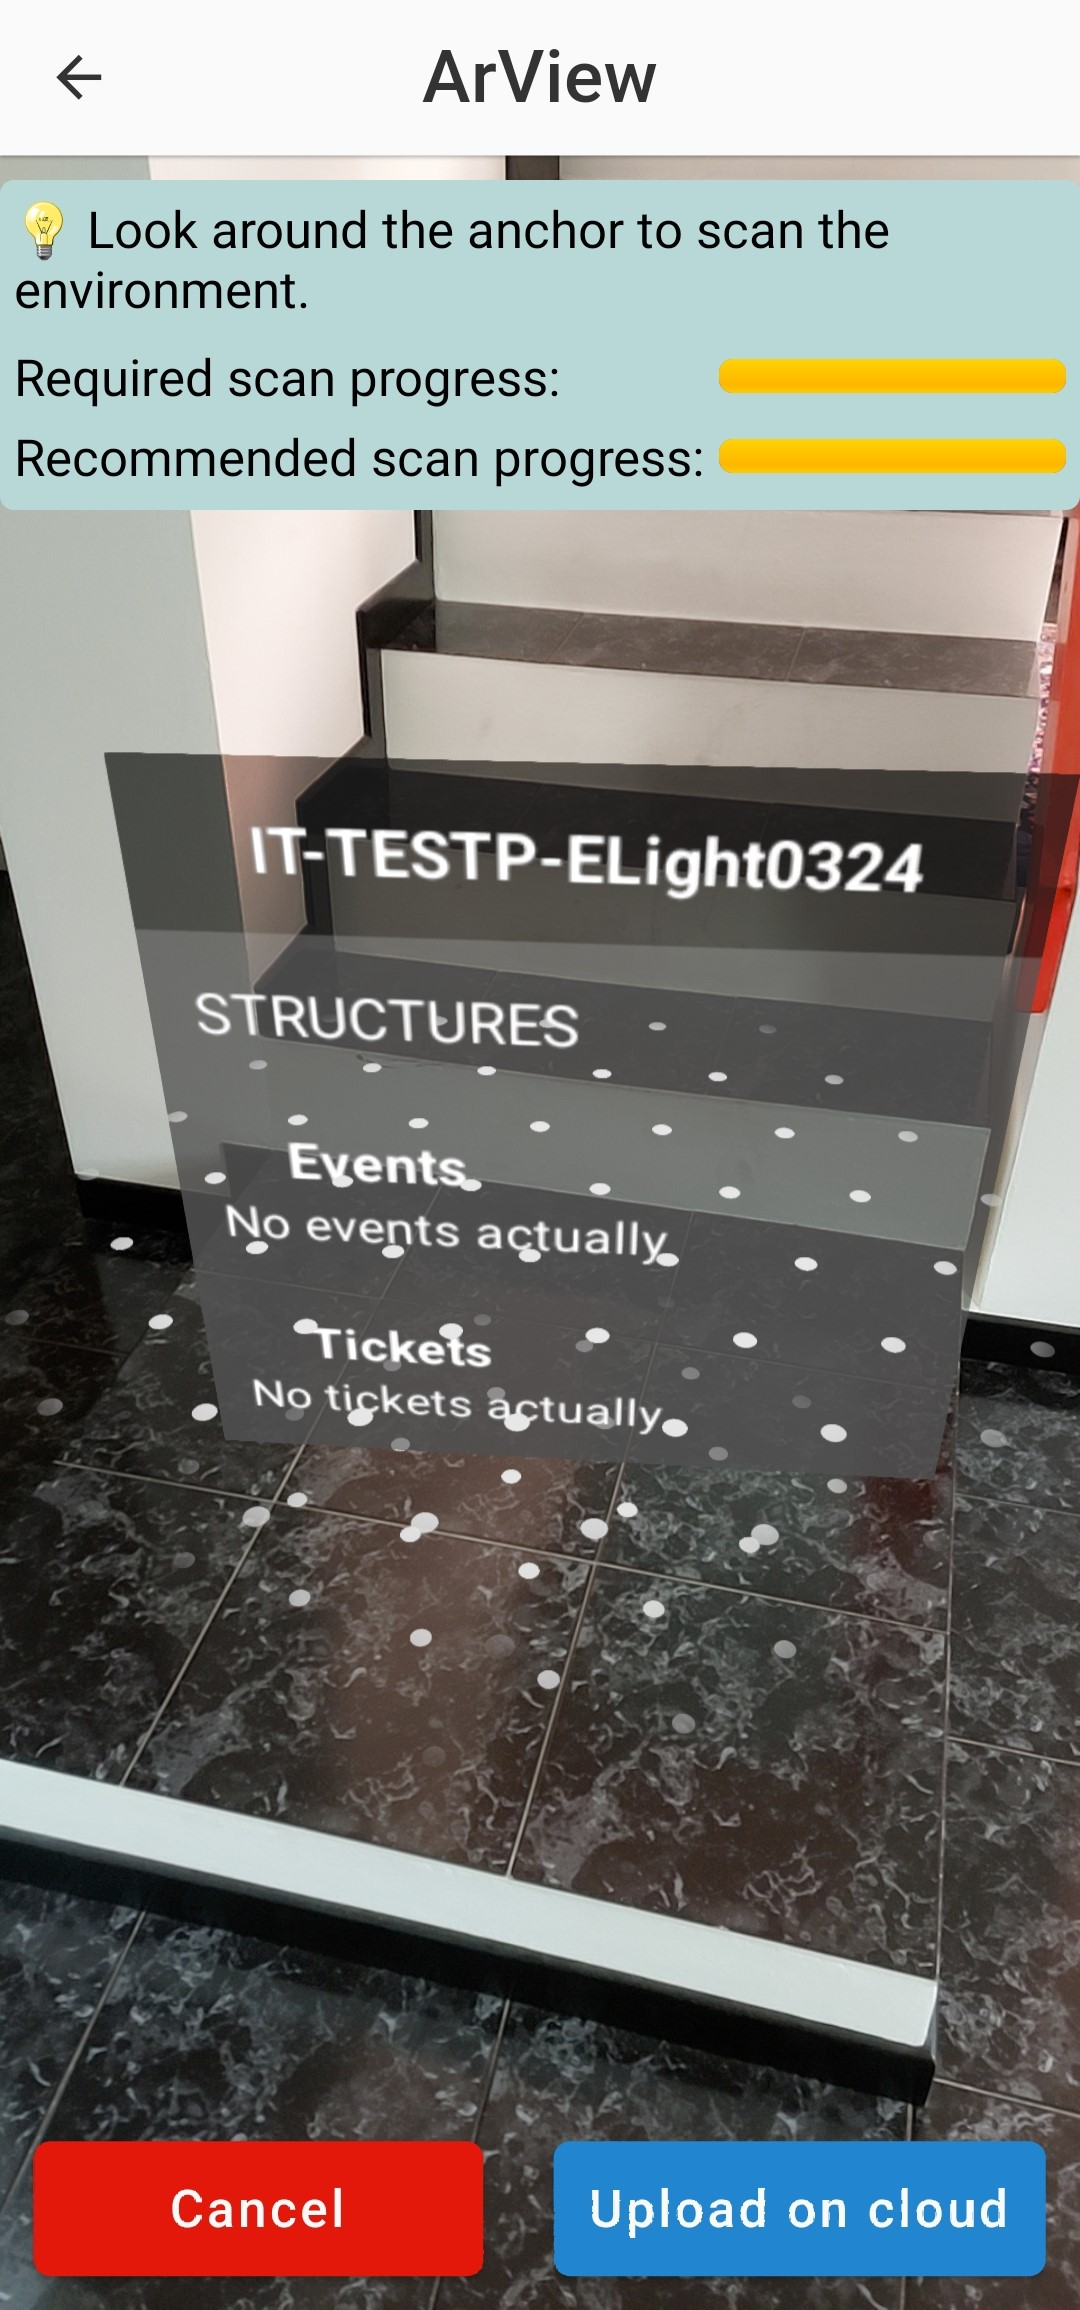
\includegraphics[width=.3\textwidth]{place_asset_scanLevel}\hfill
  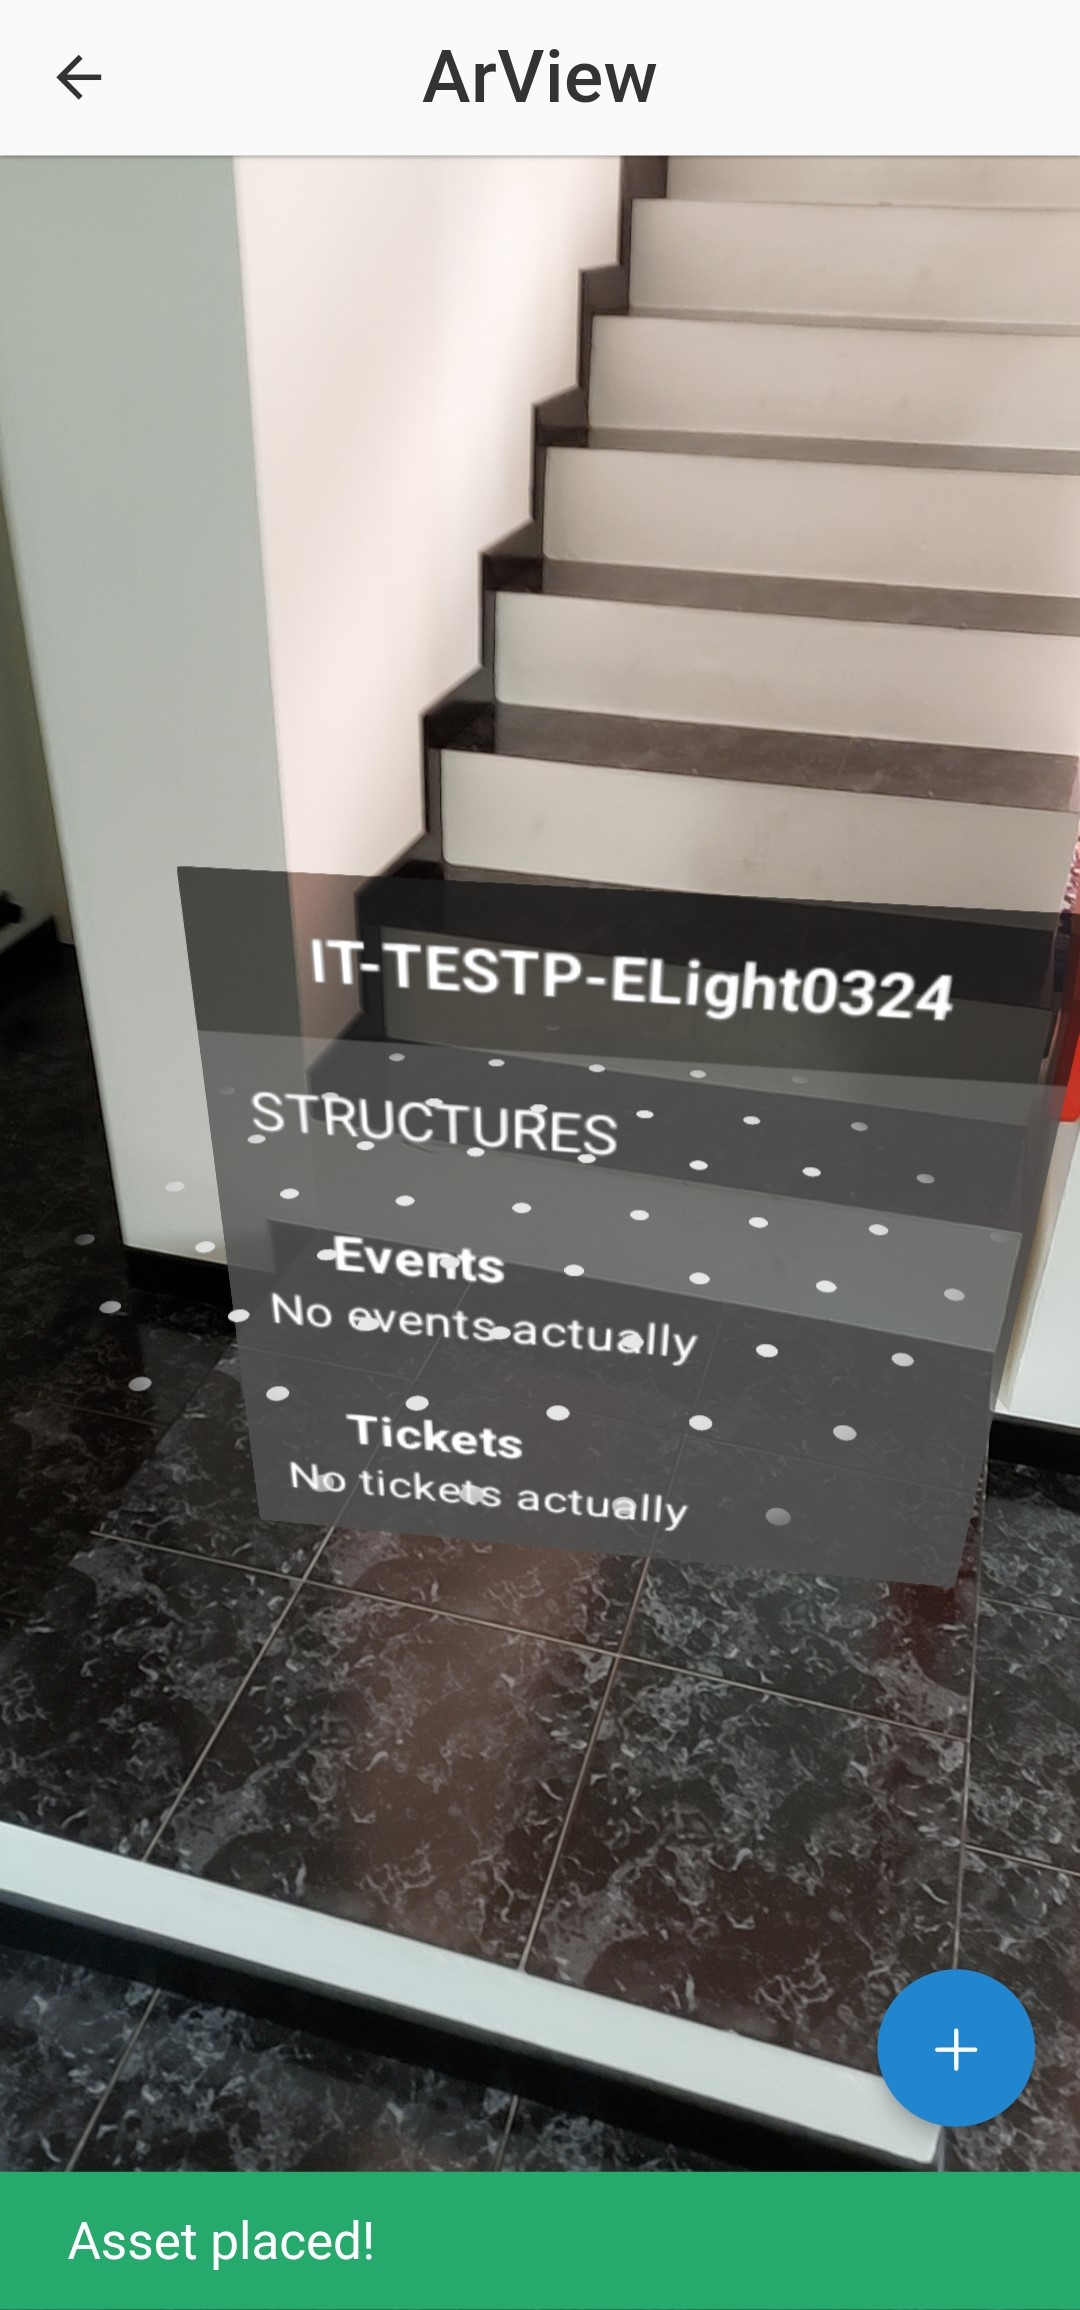
\includegraphics[width=.3\textwidth]{place_asset}\hfill
  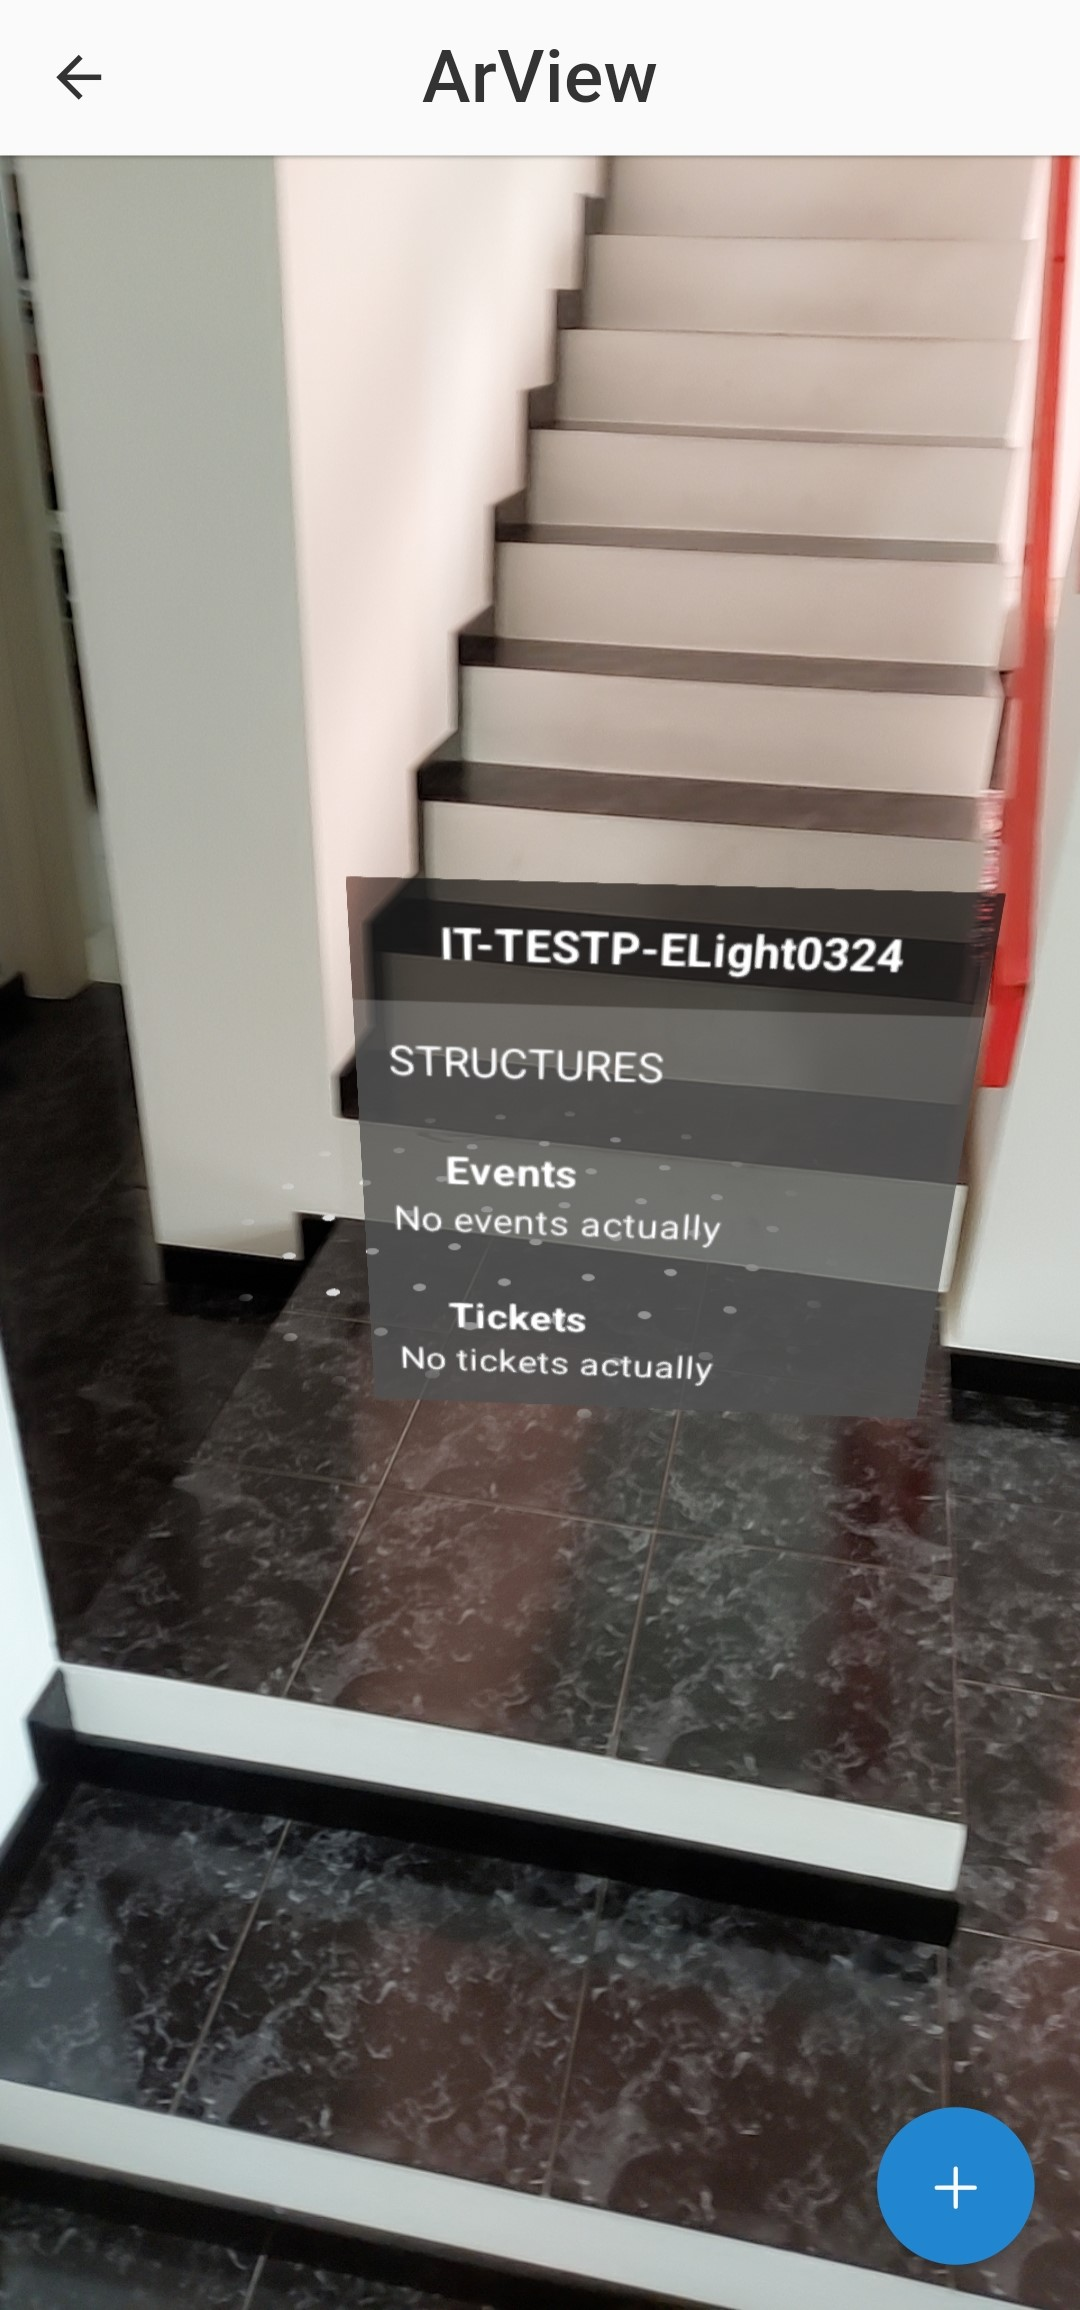
\includegraphics[width=.3\textwidth]{retrieve_asset}\hfill

  \caption[Creazione, caricamento e recupero di \textit{asset}]{In ordine: \textit{asset} viene posizionato e viene mostrato il livello di \textit{scan} dell'ambiente, viene caricato e, previa chiusura e riapertura della vista, viene recuperato dal \textit{cloud}.}
  \label{fig:place_asset}
\end{figure}

{
    \setlength{\freewidth}{\dimexpr\textwidth-10\tabcolsep}
    \renewcommand{\arraystretch}{1.5}
    \centering
    \setlength{\aboverulesep}{0pt}
    \setlength{\belowrulesep}{0pt}
    \rowcolors{2}{red!10}{white}
    \begin{longtable}{C{.15\freewidth} C{.965\freewidth}}
       \toprule
    \rowcolor{red}
    \textcolor{white}{\textbf{Codice}}&
    \textcolor{white}{\textbf{Descrizione}}\\
    \toprule
    \endhead

    R1F1 & Il \textit{plugin} deve rappresentare \textit{asset} tramite ancoraggio in realtà aumentata\\
    R1F11 & \textit{On-Tap} sullo spazio permette di creare una ancoraggio in posizione\\
    R1F11.1 & Ancoraggio posizionato nello spazio può essere salvato\\
    R1F11.2 & Ancoraggio posizionato nello spazio può essere eliminato\\
    R1F12 & Il salvataggio di un ancoraggio è disponibile solo quando è sicuro vada a buon fine\\
    R1F12.1 & Viene mostrato a schermo un feedback riguardo il livello di sicurezza raggiunto\\

    \bottomrule
    \rowcolor{white} 
    \caption{Requisiti soddisfatti in figura \ref{fig:place_asset}}
    \end{longtable}
}

Effettuando un \textit{On-Tap} su un ancoraggio appare una \textit{bottom sheet} che mostra l'identificatore dell'\textit{asset} e, se ci sono, gli eventi e i \textit{ticket} aperti a lui associati. Permette inoltre di raggiungere i dettagli dell'\textit{asset} o di rimuoverlo.\\
Poi, nella lista degli \textit{asset} disponibili, quelli già collegati a un ancoraggio in realtà aumentata presentano un piccolo marcatore con dicitura "AR", permettendo di raggiungere la vista con il bottone a forma di cubo in altro a destra. E' grigio perché l'uso richiederebbe di essere fisicamente presenti in "Plant 1" e di selezionare inoltre stabilimento, piano e stanza.

\begin{figure}[H]
  \centering
  %\includegraphics[height=5cm]{screen_mobilesyn}
  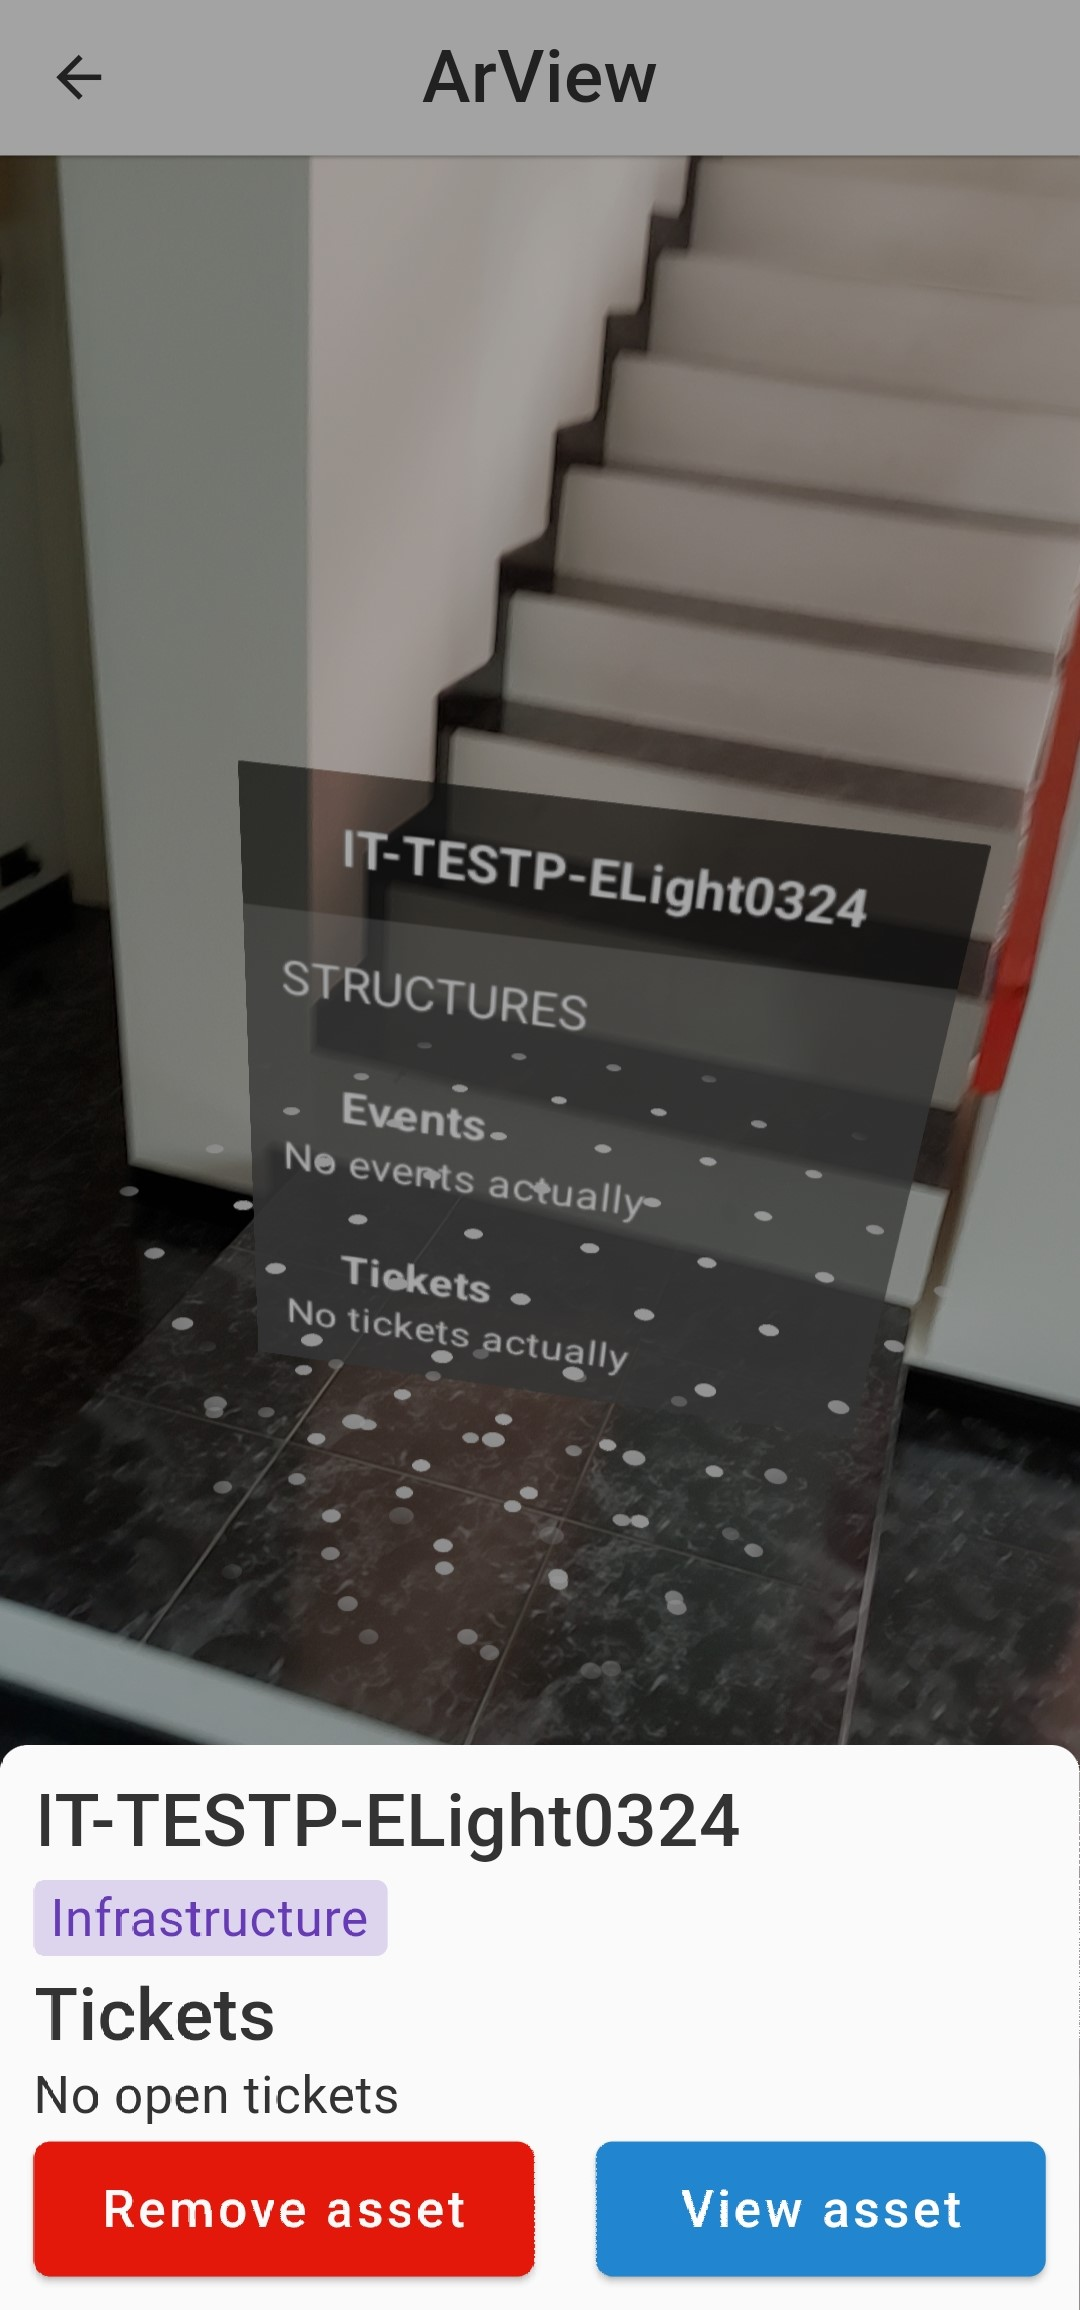
\includegraphics[width=.3\textwidth]{asset_card_onTap}\hfill
  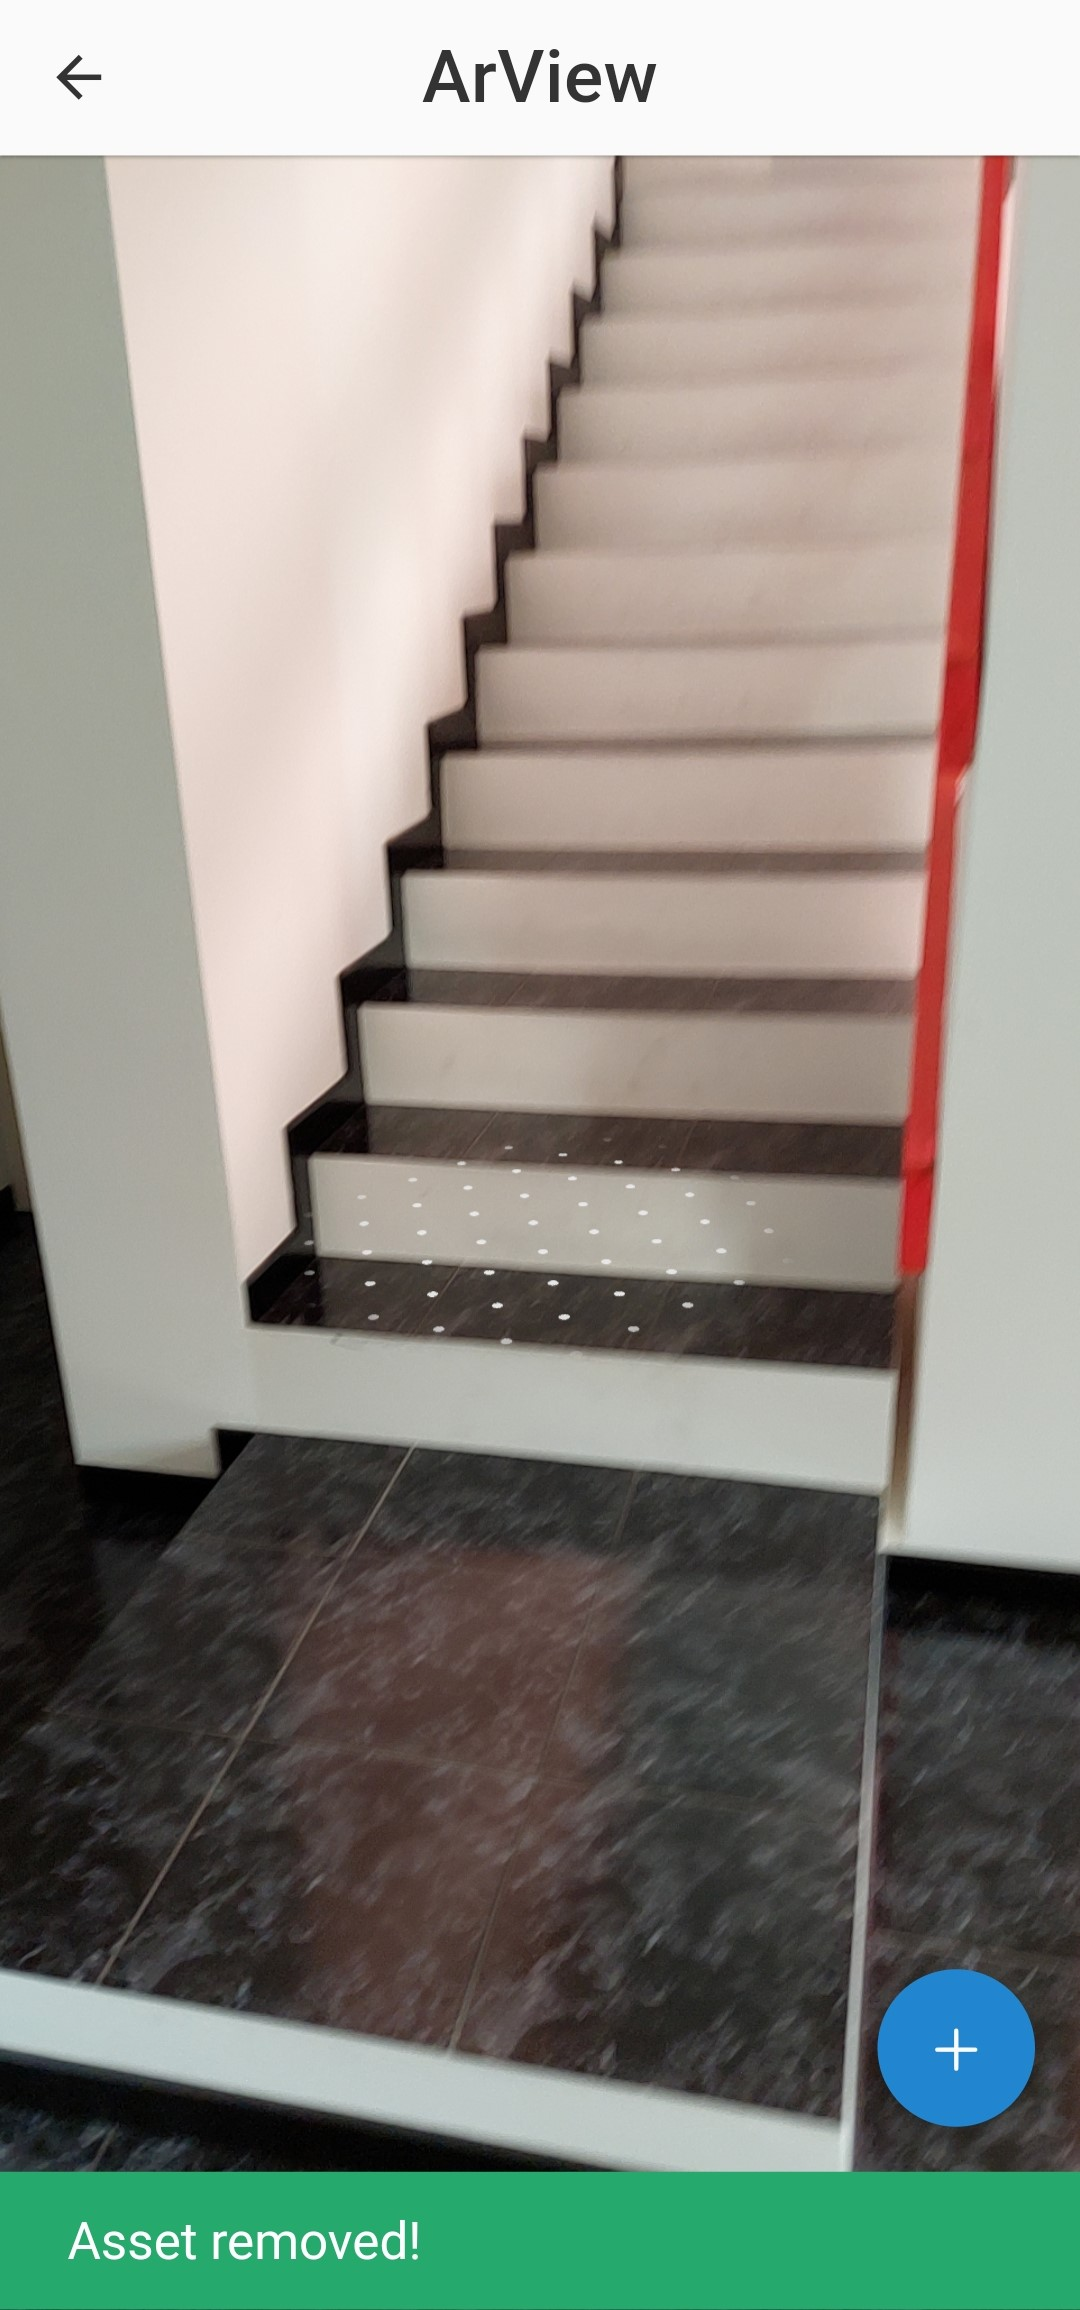
\includegraphics[width=.3\textwidth]{remove_asset}\hfill
  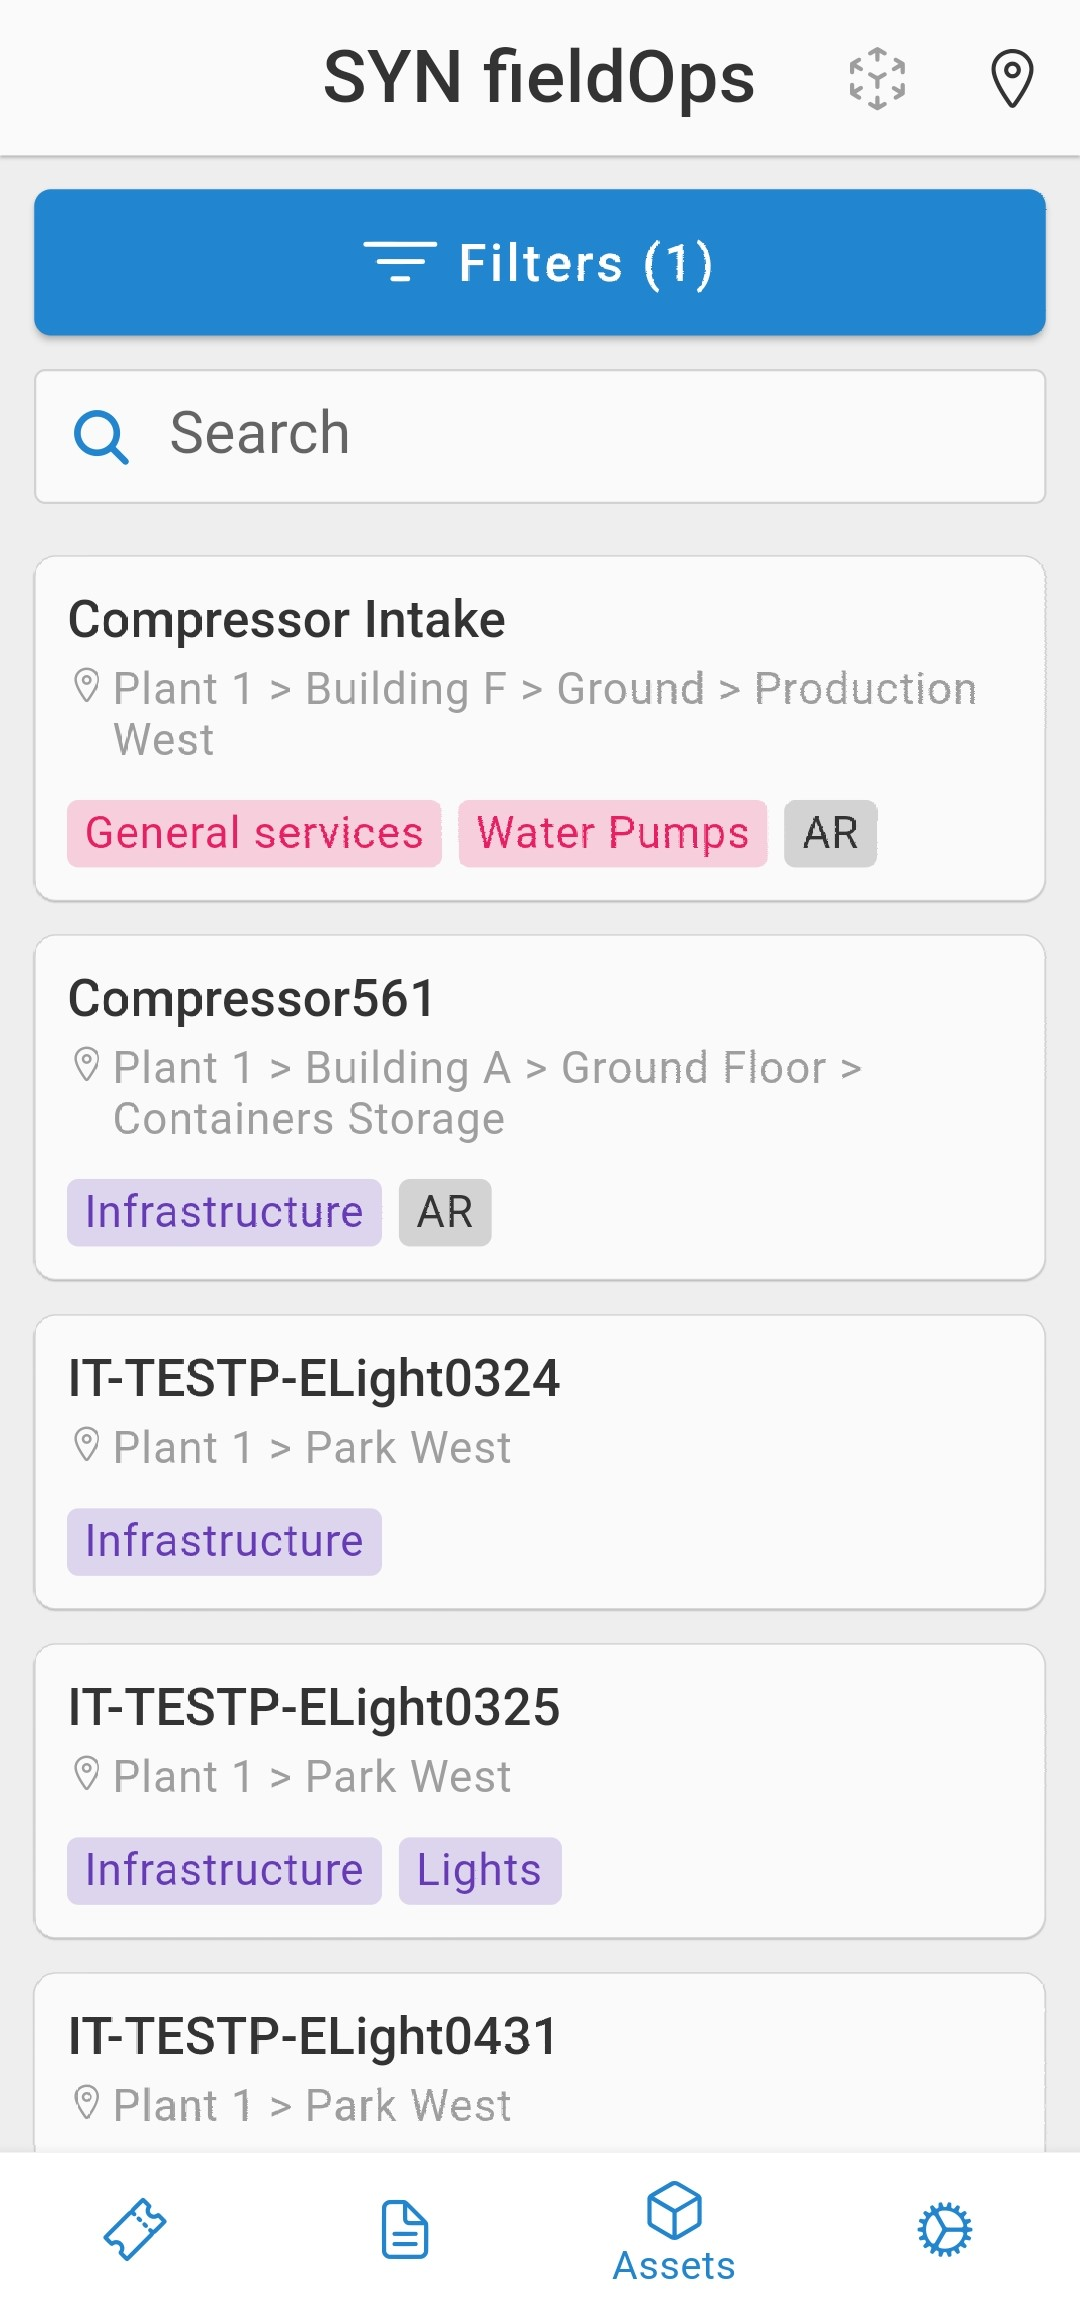
\includegraphics[width=.3\textwidth]{asset_list}
  \caption[\textit{Bottom sheet asset} per eliminazione e lista \textit{asset}]{\textit{Bottom sheet} per l'\textit{asset} "IT-TESTP-ELight0324" e successiva eliminazione tramite bottone con dicitura \textit{"Remove Asset"}. L'ultima immagine mostra invece la lista degli \textit{asset} presenti con il bottone per raggiungere la vista in realtà aumentata.}
  \label{fig:asset_list}
\end{figure}

{
    \setlength{\freewidth}{\dimexpr\textwidth-10\tabcolsep}
    \renewcommand{\arraystretch}{1.5}
    \centering
    \setlength{\aboverulesep}{0pt}
    \setlength{\belowrulesep}{0pt}
    \rowcolors{2}{red!10}{white}
    \begin{longtable}{C{.15\freewidth} C{.965\freewidth}}
       \toprule
    \rowcolor{red}
    \textcolor{white}{\textbf{Codice}}&
    \textcolor{white}{\textbf{Descrizione}}\\
    \toprule
    \endhead

    R1F5 & Utente deve poter vedere quali \textit{asset} hanno ancoraggio associato\\
    R1F7 & Utente deve poter raggiungere la vista in realtà aumentata dalla schermata degli \textit{asset}\\
    R1F8 & \textit{On-Tap} su una ancoraggio deve aprire una \textit{bottom sheet} contestuale\\
    R1F8.1 & \textit{Bottom sheet} deve presentare identificatore per \textit{asset} o \textit{ticket} associato all'ancoraggio\\
    R1F8.2 & \textit{Bottom sheet} associato a un \textit{asset} mostra \textit{ticket} aperti se presenti\\
    R1F8.3 & \textit{Bottom sheet} deve fornire \textit{Call-To-Action} per eliminare l'ancoraggio\\
    R1F8.4 & \textit{Bottom sheet} deve fornire \textit{Call-To-Action} per raggiungere pagina di dettaglio\\
    

    \bottomrule
    \rowcolor{white} 
    \caption{Requisiti soddisfatti in figura \ref{fig:asset_list}}
    \end{longtable}
}

Per quanto riguarda i \textit{ticket} invece l'approccio scelto è quello di far apparire, al completamento della compilazione di un \textit{ticket}, una finestra che permette di posizionarlo in realtà aumentata. In questo caso si può notare la \textit{card} di stato aggiornata per quanto riguarda la notifica del livello di \textit{scan} per il caricamento dell'ancoraggio.\\
Mostriamo inoltre che i \textit{ticket} aperti di un \textit{asset} mettono in chiaro data e ora di apertura.

\begin{figure}[H]
  \centering
  %\includegraphics[height=5cm]{screen_mobilesyn}
  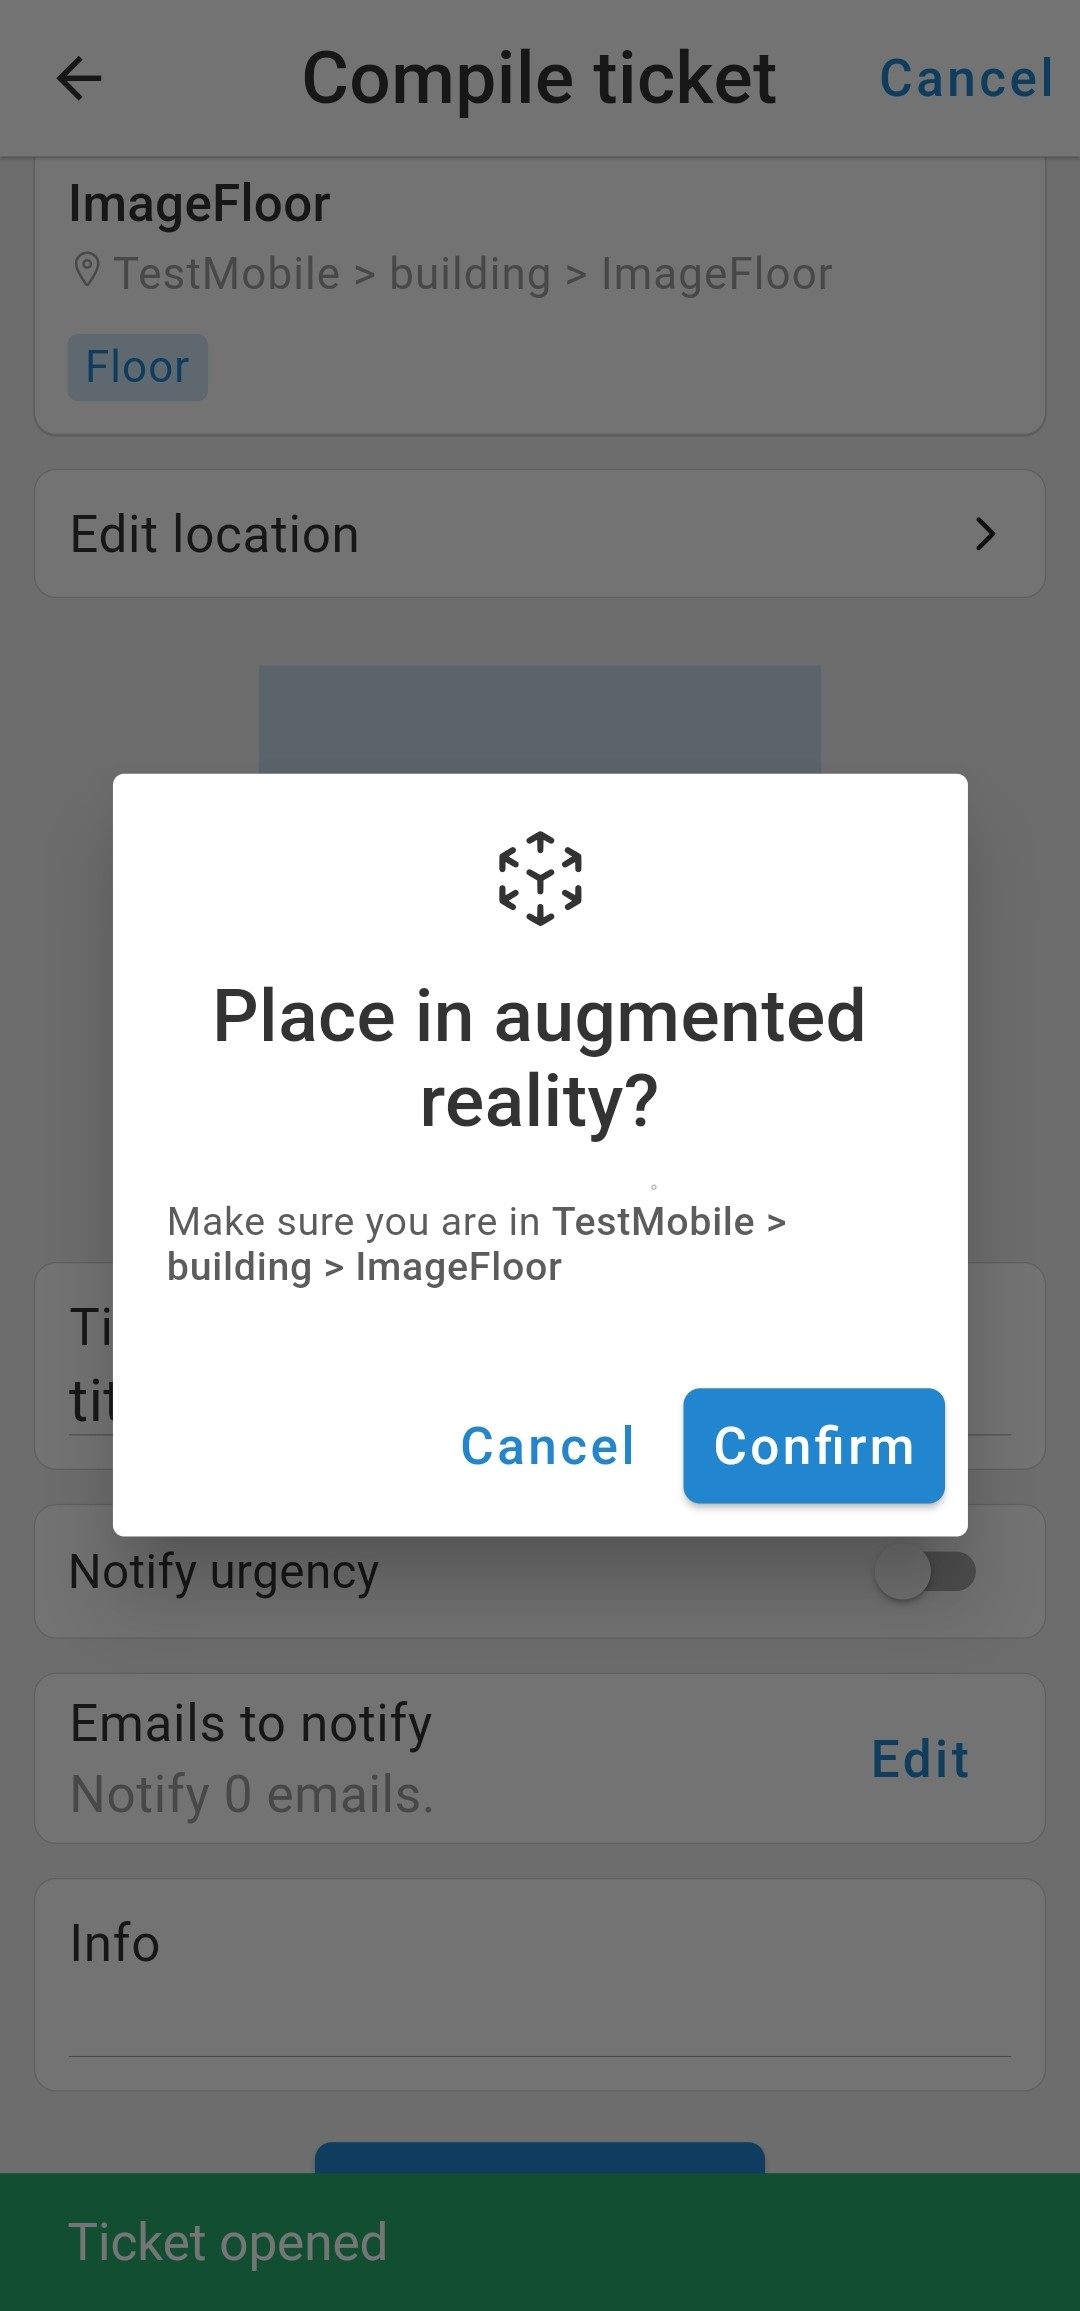
\includegraphics[width=.3\textwidth]{ticket_ar1}\hfill
  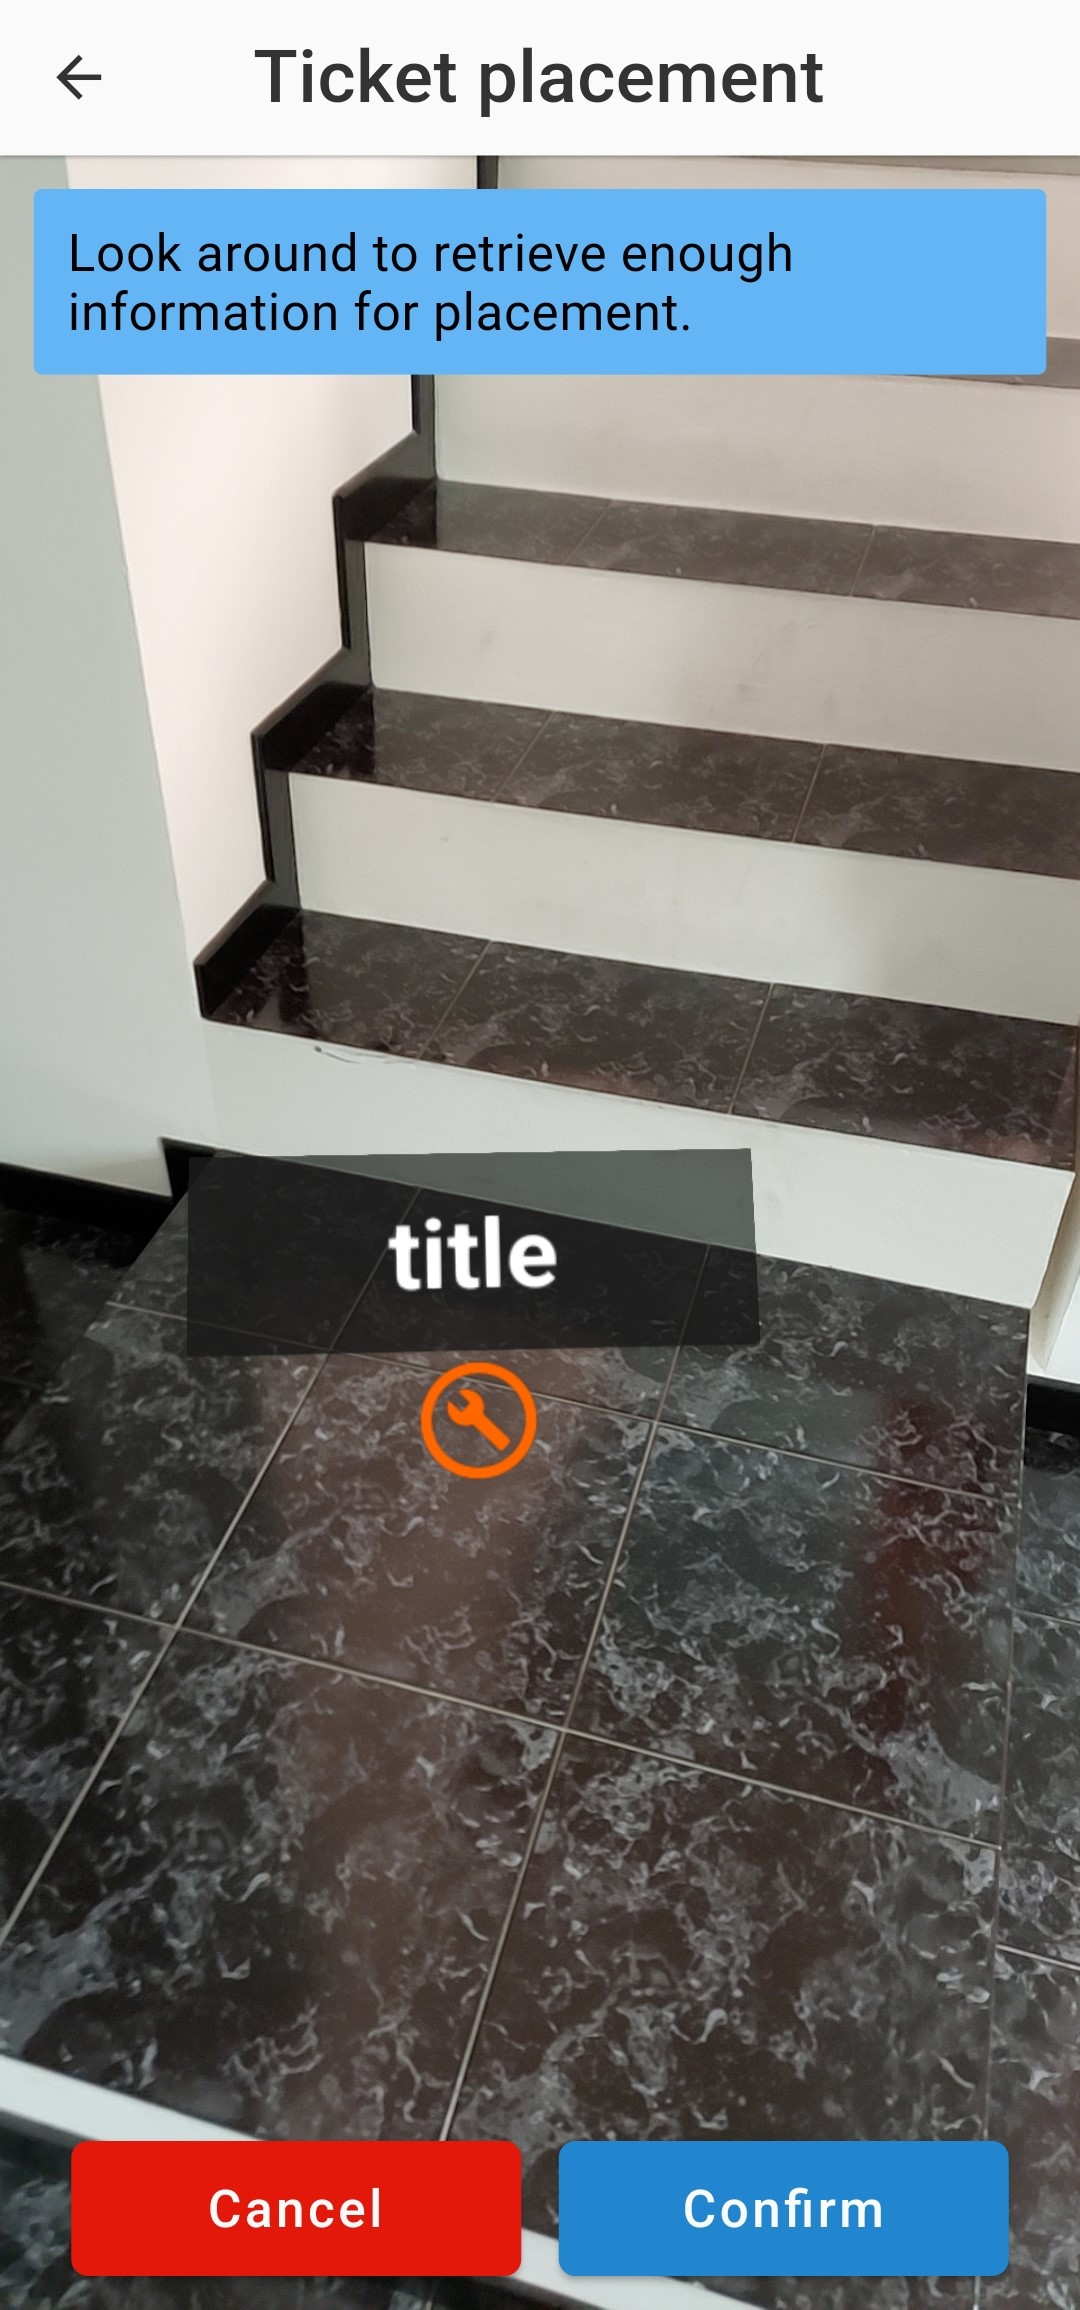
\includegraphics[width=.3\textwidth]{ticket_ar2}\hfill
  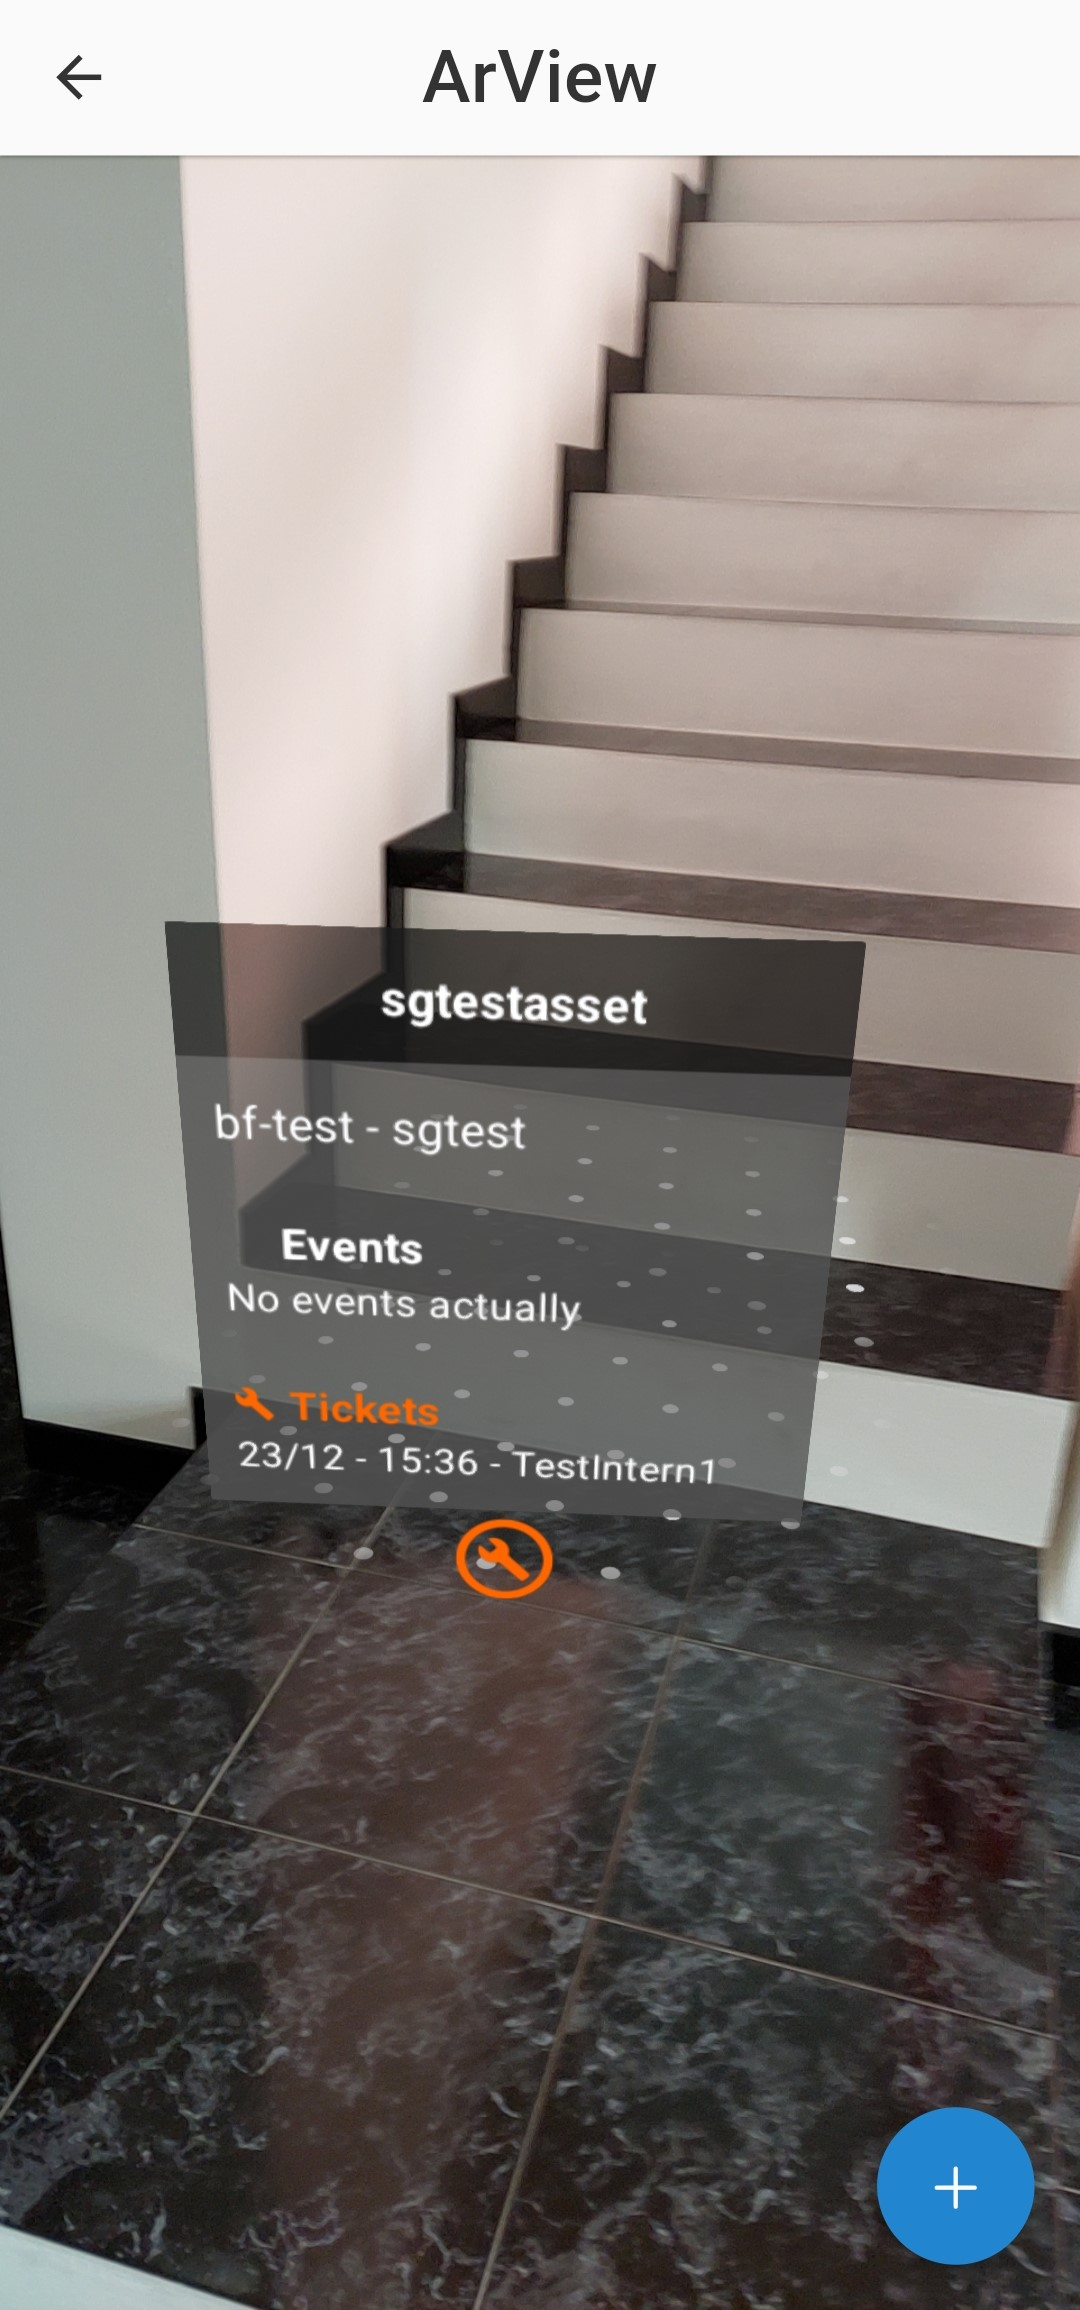
\includegraphics[width=.3\textwidth]{asset_with_ticket}
  \caption[Caricamento \textit{ticket} realtà aumentata e \textit{ticket} su \textit{asset}]{Una volta compilato il \textit{ticket} appare una finestra in sovrimpressione che permette di posizionarlo in realtà aumentata. Inoltre i \textit{ticket} di un \textit{asset} mostrano data e ora di apertura.}
  \label{fig:ticket_ar}
\end{figure}

{
    \setlength{\freewidth}{\dimexpr\textwidth-10\tabcolsep}
    \renewcommand{\arraystretch}{1.5}
    \centering
    \setlength{\aboverulesep}{0pt}
    \setlength{\belowrulesep}{0pt}
    \rowcolors{2}{red!10}{white}
    \begin{longtable}{C{.15\freewidth} C{.965\freewidth}}
       \toprule
    \rowcolor{red}
    \textcolor{white}{\textbf{Codice}}&
    \textcolor{white}{\textbf{Descrizione}}\\
    \toprule
    \endhead

    R1F2 & Il \textit{plugin} deve rappresentare \textit{ticket} tramite ancoraggio in realtà aumentata\\
    R1F9 & Le informazioni contestuali di un \textit{ticket} includono data e ora di creazione\\
    R1F10 & Gli ancoraggi hanno rappresentazione visiva contestuale\\ 
  
    \bottomrule
    \rowcolor{white} 
    \caption{Requisiti soddisfatti in figura \ref{fig:ticket_ar}}
    \end{longtable}
}



